\documentclass[uplatex,dvipdfmx,a4paper,11pt]{jsarticle}

\usepackage{docmute}


% 数式
\usepackage{amsmath,amsthm,amssymb}
\usepackage{bm}
% 画像
\usepackage{graphicx}

\usepackage{multirow}
\usepackage{wrapfig}
\usepackage{ascmac}
\usepackage{xcolor}


\usepackage{makeidx}
\makeindex

\graphicspath{{../../_Figures//}{../../_Figures/Rheology/}}

\usepackage{qrcode}
\setlength\lineskiplimit{0pt}
\setlength\normallineskiplimit{0pt}

\usepackage{qexam}

\usepackage{titlesec}
\titleformat*{\section}{\Large\bfseries}
\titleformat*{\subsection}{\large\bfseries}
\titleformat*{\subsubsection}{\normalsize\bfseries}
\titleformat*{\paragraph}{\normalsize\bfseries}

% ページ設定
% \pagestyle{empty}
% 高さの設定
\setlength{\textheight}{\paperheight}   % ひとまず紙面を本文領域に
\setlength{\topmargin}{-5.4truemm}      % 上の余白を20mm(=1inch-5.4mm)に
\addtolength{\topmargin}{-\headheight}  % 
\addtolength{\topmargin}{-\headsep}     % ヘッダの分だけ本文領域を移動させる
\addtolength{\textheight}{-40truemm}    % 下の余白も20mmに%% 幅の設定
\setlength{\textwidth}{\paperwidth}     % ひとまず紙面を本文領域に
\setlength{\oddsidemargin}{-5.4truemm}  % 左の余白を20mm(=1inch-5.4mm)に
\setlength{\evensidemargin}{-5.4truemm} % 
\addtolength{\textwidth}{-40truemm}     % 右の余白も20mmに
% 図と本文との間
%\abovecaptionskip=-5pt
%\belowcaptionskip=-5pt
%
% 全体の行間調整
% \renewcommand{\baselinestretch}{1.0} 
% 図と表
%\renewcommand{\figurename}{Fig.}
%\renewcommand{\tablename}{Tab.}
%

% \makeatletter 
% \def\section{\@startsection {section}{1}{\z@}{1.5 ex plus 2ex minus -.2ex}{0.5 ex plus .2ex}{\large\bf}}
% \def\subsection{\@startsection{subsection}{2}{\z@}{0.2\Cvs \@plus.5\Cdp \@minus.2\Cdp}{0.1\Cvs \@plus.3\Cdp}{\reset@font\normalsize\bfseries}}
% \makeatother 

\usepackage[dvipdfmx,%
 bookmarks=true,%
 bookmarksnumbered=true,%
 colorlinks=false,%
 setpagesize=false,%
 pdftitle={数式に頼らない直感的理解による材料設計のためのレオロジー⼊⾨},%
 pdfauthor={佐々木裕},%
 pdfsubject={},%
 pdfkeywords={レオロジー; 材料設計; }]{hyperref}
\usepackage{pxjahyper}

\usepackage{plext}

\usepackage{niceframe} 
\usepackage{framed}
\newenvironment{longartdeco}{%
  \def\FrameCommand{\fboxsep=\FrameSep \artdecoframe}%
  \MakeFramed {\FrameRestore}}%
 {\endMakeFramed}
 
\usepackage{siunitx}

\newcommand{\rmd}{\mathrm{d}}

\usepackage[inline]{showlabels}

\begin{document}

\section*{この章の内容}

この章では、物質の三態(固体、液体、気体)という最も基本的な「ものの有り様」について、物理化学的に⾒直していきます。

まず、固体を粒子が整列した結晶モデルでイメージして、その弾性体としての力の起源がどのように生じているのかを理解します。
そして、液体が流れるということを、マクロな変形が粒子モデルでのミクロな移動にどのようにつながるかというイメージを深めたうえで、
固体と液体の違い、さらには、その間に存在するガラス状態を理解していきます。

最後に、刺激の応答としての応⼒がどのように発⽣するのかということについて、固体の場合と液体の場合のそれぞれのあり方をイメージできるようにします。

具体的に列記すると、以下のような事項となります。
\begin{boxnote}
	\large
    \begin{itemize}
		\item 物質の三態について
		\begin{itemize}
			\item 固体のモデルとしての結晶
			\item 液体のモデル
		\end{itemize} 
		\item 流れるということは?
		\begin{itemize}
			\item マクロな変形と粒子の移動
			\item 固体と液体の境目
			\item ガラス状態
		\end{itemize} 
		\item 応力の由来は?
		\begin{itemize}
			\item 結晶の応力の起源
			\item 液体の応力とは?
		\end{itemize}
	\end{itemize}
\end{boxnote}

\section{物質の三態について}

\subsection{物質の三態}
物質の状態は、その相の違いによって固体\index{こたい@固体}、液体\index{えきたい@液体}、気体の3つに分類できます。
これから、その由来について考えていきましょう。
\begin{figure}[htb]
	\begin{center}
		\begin{minipage}{0.4\textwidth}
			\large
			\begin{itembox}[l]{マクロとミクロに考えて、}
				\begin{itemize}
					\item マクロな視点では?
					\begin{itemize}
						\item 気体、液体 ⇔ 流れる
						\item 固体 ⇔ 流れない
					\end{itemize}
					\item ミクロに中身を考えると、\\何が違うのでしょうか?
				\end{itemize}
			\end{itembox}
		\end{minipage}
		\begin{minipage}{0.5\textwidth}
			\begin{center}
			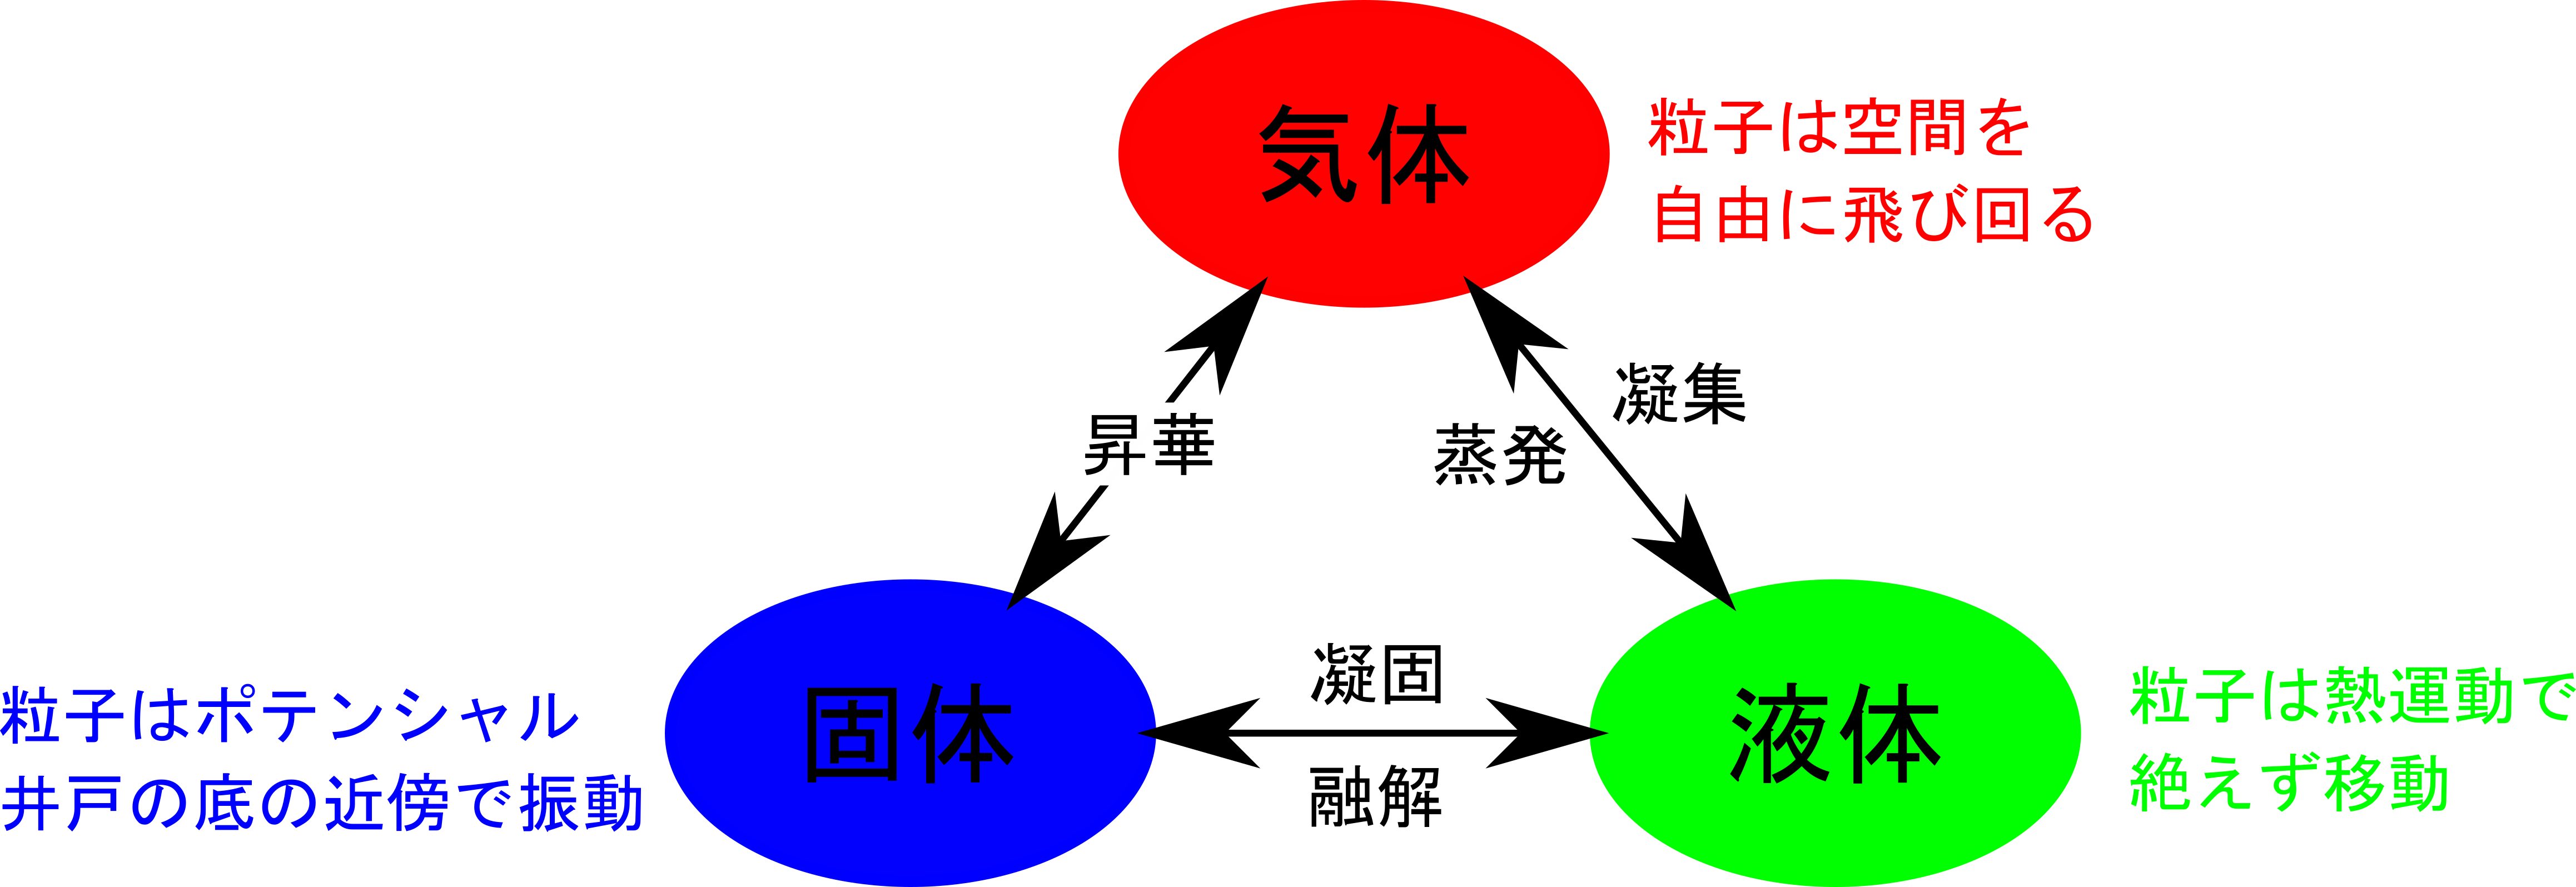
\includegraphics[width=\textwidth]{3Phase.png}
			\end{center}
		\end{minipage}
		\caption{物質の三態について}
		\label{fig:santai}
	\end{center}
\end{figure}

\subsubsection{ミクロとマクロ}
歴史的に考えると、物質の状態は人間が手で触って実感できるようなマクロな性質に従って、分類されてきました。
すなわち、固体\index{こたい@固体}は定まった体積と形を持つ物体であり、一方、液体\index{えきたい@液体}は体積を減少させるように押しつぶすことは困難ですが、
形は自由に変化します。
そして、気体では圧縮することもできるので体積も形も定まっていないという性質を持っています。

雰囲気温度が変化すれば、それに応じて、物質はこの三態の間を移ろっていきます。
物質が置かれている環境の温度を低下させれば、気体は凝集して液体\index{えきたい@液体}となり、液体\index{えきたい@液体}は凝固して固体\index{こたい@固体}となります。
逆に、固体\index{こたい@固体}を温度が高い状態とすれば融解して液体\index{えきたい@液体}になり、さらなる加熱により液体\index{えきたい@液体}が蒸発して気体へと変化します。

この三態の振る舞いをレオロジー的に考えると、「流れるかどうか」ということが重要なポイントになります。
すなわち、液体\index{えきたい@液体}と固体\index{こたい@固体}との明白な相違点は流れるかどうかということに集約されるわけです。

そして、「流れるという現象」を考えていく場合には、物質の内部のミクロな状態を考える必要が出てきます。
ミクロな視点に立った場合に、流れるという現象はどのように考えることができるのでしょうか。

\subsection{固体\index{こたい@固体}のモデルとしての結晶}
まず、出発点として、固体\index{こたい@固体}のモデルを考えていきましょう。

前述のように、固体\index{こたい@固体}の特徴は流れないということでした。
この特性は、ミクロにはどのようなモデルとして考えれば理解できるのでしょうか。

\subsubsection{結晶のモデル}
マクロに見た固体\index{こたい@固体}を具体的に考えると、金属、塩、鉱物(石)、セラミックス(陶器)、ガラス、木材、等々に分類されます。
これらの物質は、その成り立ちが違うため、それを構成する物質の組成も全く異なったものとなっています。

簡略化して取り扱うために、中学や高校で習ったような物理化学の範囲においては思い切った単純化を行って、
固体\index{こたい@固体}は何らかの粒子\index{りゅうし@粒子}(原子や分子)が規則的に並んだ「結晶としてモデル化」されてきました。

\begin{figure}[htb]
	\begin{center}
		
\includegraphics[width=.9\textwidth]{crystals.png}
		\caption{結晶という固体の模式図}
		\label{fig:crystals}
	\end{center}
\end{figure}

\subsubsection{二粒子間のポテンシャル}

個体を、粒子\index{りゅうし@粒子}が規則的に整列することによって構成されたと考える結晶構造としてモデル化した場合、
マクロに見たときの「流れないという性質」は、ミクロに見れば粒子間に強い相互作用が働いているということに対応します。
つまり、粒子間に隣の粒子\index{りゅうし@粒子}を引き止めるような力が働いているおかげで、マクロな性質である形状維持して流れないという特性が生じていると
考えるわけです。
\begin{figure}[htb]
	\begin{center}
		\begin{minipage}{0.4\textwidth}
			\large
			\begin{itembox}[l]{固体の性質をミクロに}
				\begin{itemize}
					\item 固体には、マクロな\\「流れないという性質」
					\item ミクロに見れば、粒子間に強い相互作用が必要
				\end{itemize}
			\end{itembox}
		\end{minipage}
		\begin{minipage}{0.5\textwidth}
			\begin{center}
			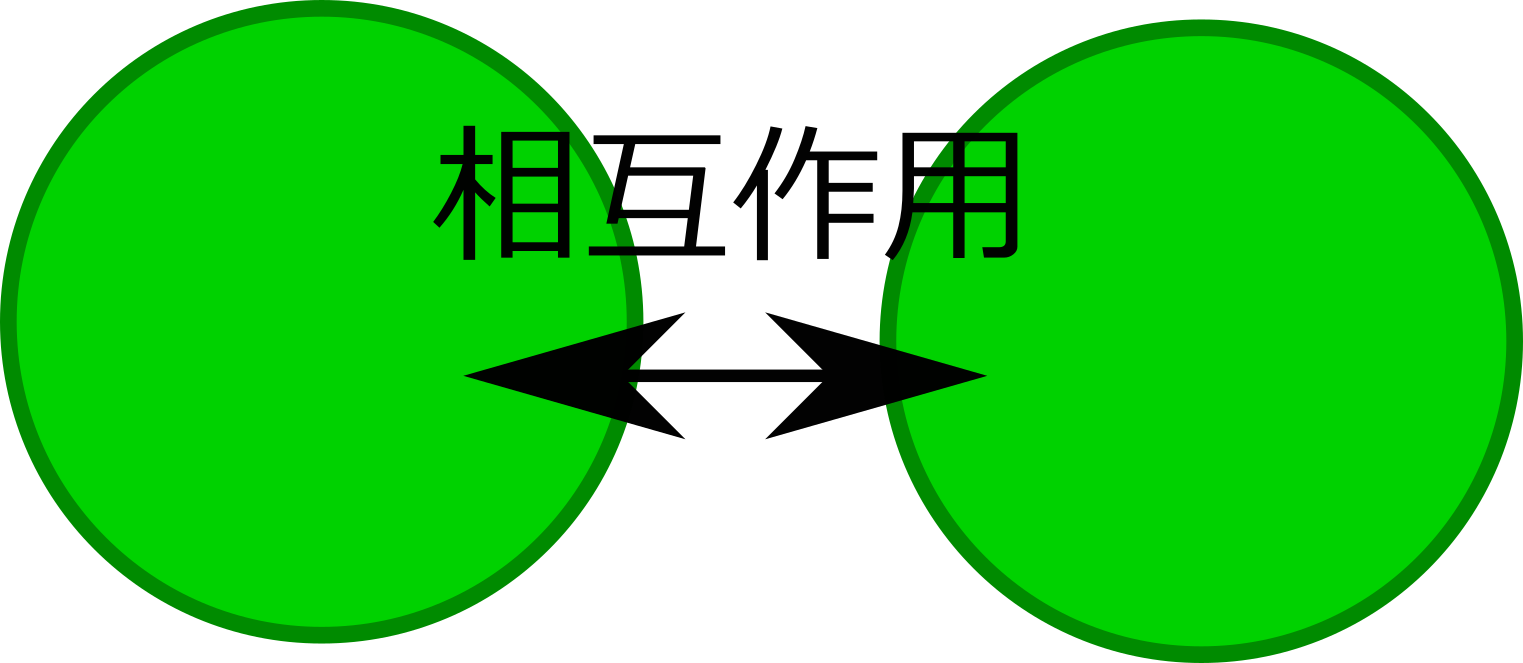
\includegraphics[width=.8\textwidth]{ryusi_1.png}
			\end{center}
		\end{minipage}
		\caption{固体を構成する粒子同士の相互作用}
		\label{fig:ryusi}
	\end{center}
\end{figure}

この粒子間の相互作用\index{そうご@相互作用}については、多様な検討が行われ、これまでに多数のモデルが提案されてきています。
その一つがよく使用されている Lennard-Jones ポテンシャル\index{れなーどじょーんずぽてんしゃる@Lennard-Jones ポテンシャル}というものになります。
\begin{figure}[htb]
	\begin{center}
		\begin{minipage}{0.4\textwidth}
			\large
			\begin{itembox}[l]{Lennard-Jones ポテンシャル}
				\begin{itemize}
					\item 速く消失する\textcolor{red}{斥力}
					\item 遠くまで働く\textcolor{blue}{引力}
					\item \textcolor{green}{それらの和}で相互作用
				\end{itemize}
				\begin{align*}
					U(r) = 4 \epsilon \left[ \textcolor{red}{\left(\dfrac{\sigma}{r} \right)^{12}} - \textcolor{blue}{\left(\dfrac{\sigma}{r} \right)^{6}} \right]
				\end{align*}
			\end{itembox}
		\end{minipage}
		\begin{minipage}{0.5\textwidth}
			\begin{center}
			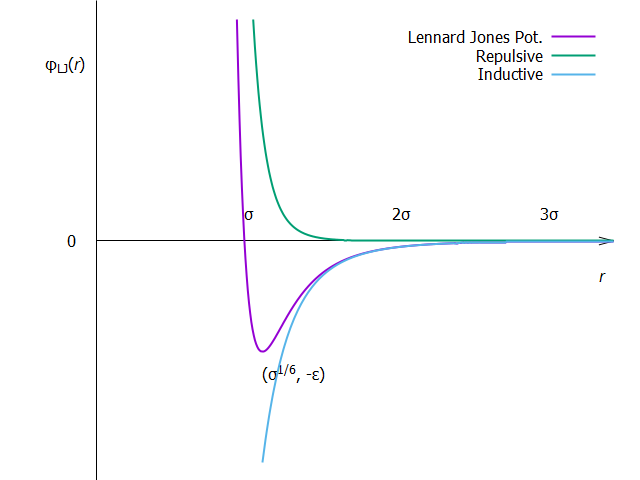
\includegraphics[width=\textwidth]{LJ_potential.png}
			\end{center}
		\end{minipage}
		\caption{Lennard-Jones ポテンシャル}
		\label{fig:Lennard-Jones}
	\end{center}
\end{figure}

これは、相対的に速く消失する斥力と遠くまで働く引力との和として二体間の相互作用\index{そうご@相互作用}を書き表したポテンシャルです。
\begin{align*}
	U(r) = 4 \epsilon \left[ \left(\dfrac{\sigma}{r} \right)^{12} - \left(\dfrac{\sigma}{r} \right)^{6} \right]
\end{align*}

以前に示したように、ポテンシャル\index{ぽてんしゃる@ポテンシャル}を微分\index{びぶん@微分}すれば、力\index{ちから@力}を表す式が得られるのでした。
したがって、上式を微分することで、粒子間に働く力 $F(r)$ がわかります。
\begin{align*}
	\begin{cases}
		U(r) = 4 \epsilon \left[ \left(\dfrac{\sigma}{r} \right)^{12} - \left(\dfrac{\sigma}{r} \right)^{6} \right] \\
		F(r) = -\dfrac{\rmd}{\rmd r}U(r) = 4 \epsilon \left[ 12 \left(\dfrac{\sigma^{12}}{r^{13}} \right) - 6 \left(\dfrac{\sigma^6}{r^7} \right) \right]
	\end{cases}
\end{align*}

このとき、ポテンシャルが極小値となるところ(ポテンシャルの井戸とも呼ぶ)において、二粒子間に働く力が 0 となっていることがわかります。
\begin{figure}[htb]
	\begin{center}
		\begin{minipage}{0.4\textwidth}
			\large
			\begin{itembox}[l]{ポテンシャルの微分で力を}
				\normalsize
				\begin{align*}
					\begin{cases}
						U(r) &= 4 \epsilon \left[ \left(\dfrac{\sigma}{r} \right)^{12} - \left(\dfrac{\sigma}{r} \right)^{6} \right] \\[10pt]
						F(r) &= -\dfrac{\rmd}{\rmd r}U(r) \\[10pt]
						&= 4 \epsilon \left[ 12 \left(\dfrac{\sigma^{12}}{r^{13}} \right) - 6 \left(\dfrac{\sigma^6}{r^7} \right) \right]
					\end{cases}
				\end{align*}
			\end{itembox}
		\end{minipage}
		\begin{minipage}{0.5\textwidth}
			\begin{center}
				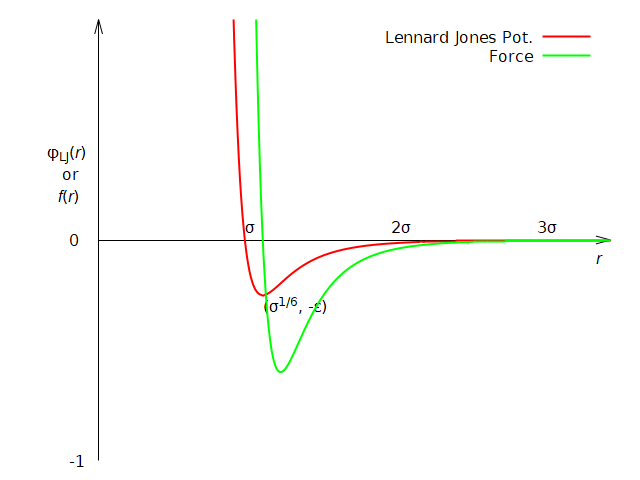
\includegraphics[width=.8\textwidth]{LJ_pot_Force.png}
			\end{center}
		\end{minipage}
		\caption{ポテンシャルの微分で力を導出}
		\label{fig:LJ_pot_Force}
	\end{center}
\end{figure}

この二粒子間に働いている力について、もう少し詳しく見てみましょう。

ポテンシャル\index{ぽてんしゃる@ポテンシャル}の極小値($r \simeq 1.16$)において二粒子間の力\index{ちから@力}は 0 となり、粒子間の距離がそれ以上に短くなると力が正となりますから、
斥力が働くことになります。
また、粒子\index{りゅうし@粒子}がその釣り合いの位置から離れすぎると力が負で引力が働きます。
これらの相互作用\index{そうご@相互作用}の結果として、二粒子間の距離がほぼ定まって、ポテンシャルの井戸の近傍に存在することが安定状態であることがわかります。
\begin{figure}[htb]
	\begin{center}
		\begin{minipage}{0.45\textwidth}
			\large
			\begin{itembox}[l]{二粒子間の力}
				\begin{itemize}
					\item 粒子の近接では斥力
					\item 離れすぎると引力
					\item その結果として、二粒子間の\\距離がほぼ定まる
				\end{itemize}
			\end{itembox}
		\end{minipage}
		\begin{minipage}{0.45\textwidth}
			\begin{center}
			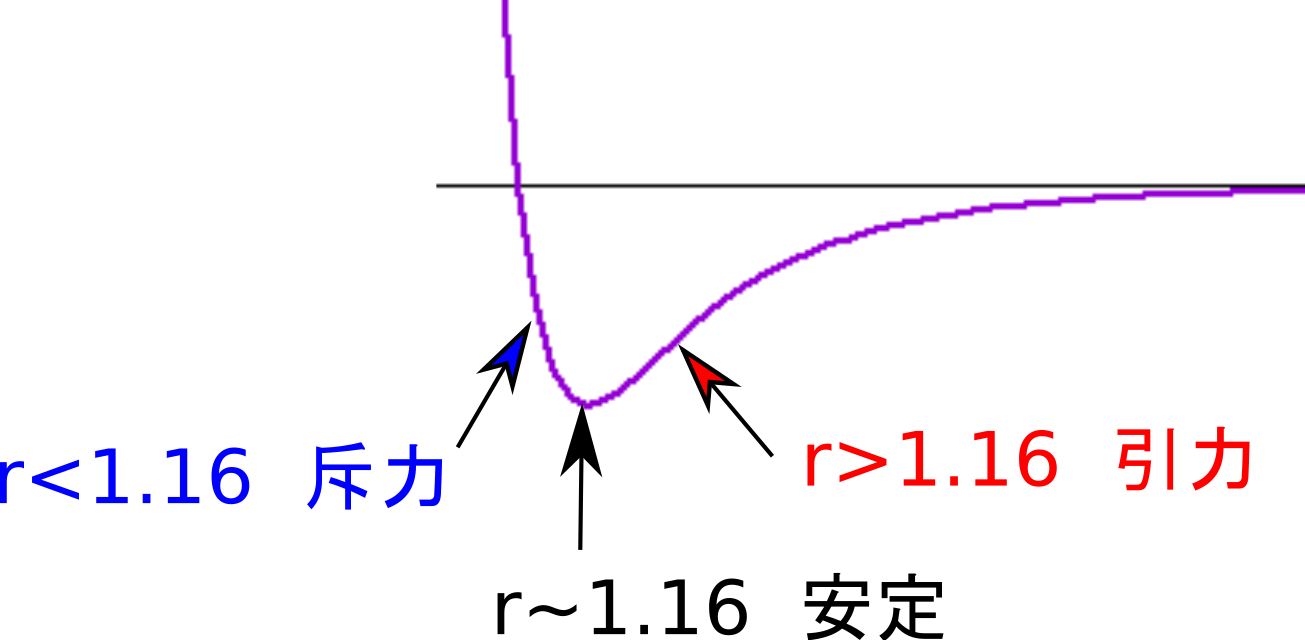
\includegraphics[width=.8\textwidth]{LJ_pos.png}
			\end{center}
		\end{minipage}
		\caption{二粒子間に働く力}
		\label{fig:lj-pos}
	\end{center}
\end{figure}

\subsubsection{多体問題として考えると、}
結晶のモデルにおいては、粒子\index{りゅうし@粒子}の相互作用\index{そうご@相互作用}は二体間に限るわけではなく、多数の粒子が相互作用\index{そうご@相互作用}を生じています。
この多体問題をきちんと解くことは大変なのですが、簡略化して安定状態を考えることもそれほど的外れではありません。
\begin{figure}[htb]
	\begin{center}
		\begin{minipage}{0.55\textwidth}
			\large
			\begin{itembox}[l]{多体系での相互作用}
				\begin{itemize}
					\item 多体の相互作用を簡略化して、
					\item 二体間の相互作用に基づくとすれば、
					\item 多体の粒子が安定距離の近傍で摂動
				\end{itemize}
			\end{itembox}
		\end{minipage}
		\begin{minipage}{0.35\textwidth}
			\begin{center}
			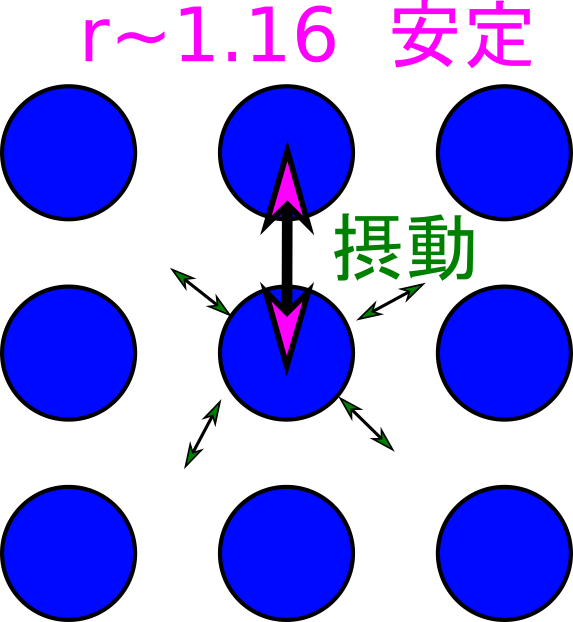
\includegraphics[width=.6\textwidth]{LJ_ryusi.png}
			\end{center}
		\end{minipage}
		\caption{簡略化した多体系の安定状態}
		\label{fig:tatai}
	\end{center}
\end{figure}

多体の相互作用\index{そうご@相互作用}を簡略化して、二体間の相互作用\index{そうご@相互作用}の単純な重ね合わせに基づくと仮定すれば、結局、
多体の粒子\index{りゅうし@粒子}が二体間相互作用の安定距離の近傍で摂動することになります。

\subsubsection{固体\index{こたい@固体}のミクロなイメージ}

二体間のポテンシャル\index{ぽてんしゃる@ポテンシャル}を用いることで、結晶モデルとして固体\index{こたい@固体}を形成する粒子の振る舞いの理解が少しだけ進みました。
ここでは、分子動力学シミュレーションという方法を使って、もう少し直感的なイメージを膨らましてみましょう。
なお、分子動力学シミュレーションの説明は以下にまとめた程度に控え、詳細は割愛します。
\large
\begin{itembox}[l]{分子動力学シミュレーションとは}
	\begin{itemize}
		\item 粒子の描像で物理現象をシミュレートする方法
		\item それぞれの粒子の運動は、ニュートン力学に従って算出する。
		\item 系の温度が粒子の揺動となる。
		\item 粒子の間に適切なポテンシャルを設定(今回は、LJ ポテンシャル)する。
	\end{itemize}
\end{itembox}
\normalsize

分子動力学シミュレーションにより、粒子間相互作用として LJ ポテンシャルを設定し、十分に低温にして固体\index{こたい@固体}における粒子の振る舞いをシミュレートした結果を、図 \ref{fig:MD-kotai} に示しました。

\begin{figure}[htb]
	\begin{center}
		\begin{minipage}{0.48\textwidth}
			\large
			\begin{itembox}[l]{固体のシミュレーション}
				\begin{itemize}
					\item T=0.1 (十分に低温な状態)
					\item 面心立方になるように、初期の\\粒子を配置。
					\item 分子動力学シミュレーションを\\実施。
					\item 動的な運動を見ても、粒子の\\動きが殆ど見られない。
				\end{itemize}
			\end{itembox}
		\end{minipage}
		\begin{minipage}{0.42\textwidth}
			\begin{center}
			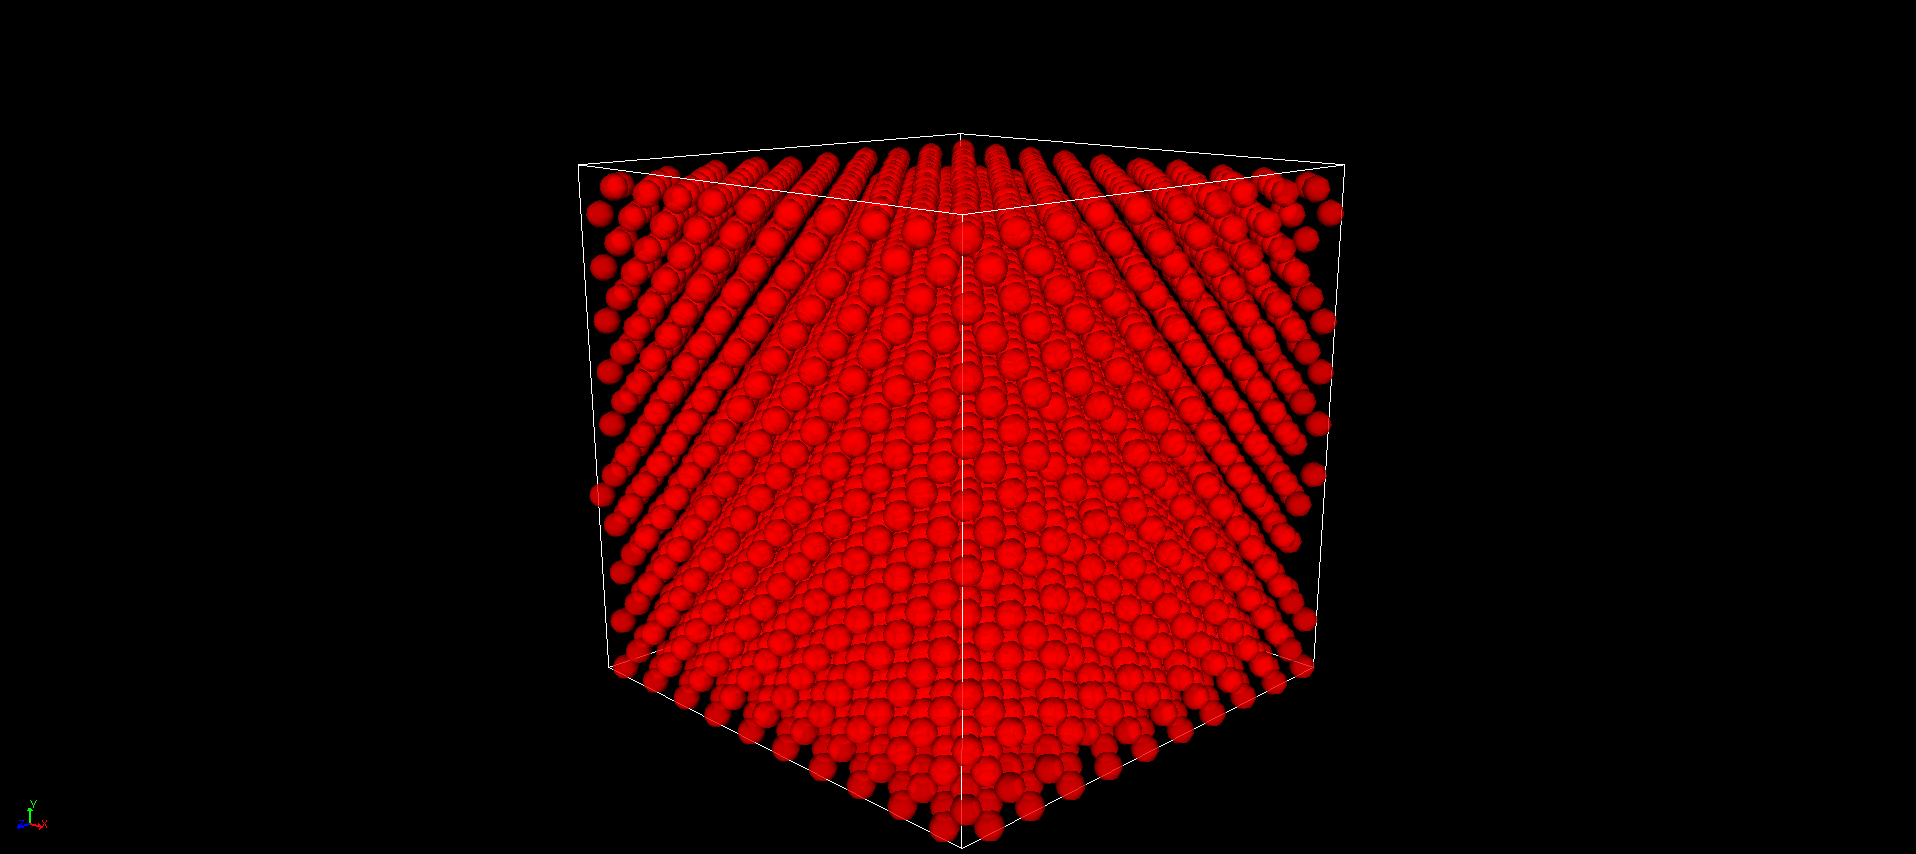
\includegraphics[width=\textwidth]{N1_FCC.png}
			\large
			\begin{screen}
				\begin{itemize}
					\item これはスナップショット
					\item 動画でも殆ど動いていない。
				\end{itemize}
			\end{screen}
			\end{center}
		\end{minipage}
		\caption{固体の分子動力学シミュレーション}
		\label{fig:MD-kotai}
	\end{center}
\end{figure}

このシミュレーションの結果として、十分に低温とした場合には粒子\index{りゅうし@粒子}の運動は抑制され、ポテンシャルの井戸の底に対応する場所でわずかに摂動する程度のものであることが確認できます。


\subsection{固体\index{こたい@固体}と液体\index{えきたい@液体}}
ここまでの議論で、固体\index{こたい@固体}のミクロなモデルの振る舞いは少しずつ理解が進んできました。
次に、固体\index{こたい@固体}と液体\index{えきたい@液体}との違いについて、シミュレーションも活用しながらイメージを膨らませていきましょう。

\subsubsection{固体\index{こたい@固体}と液体\index{えきたい@液体}の間の相転移}

固体\index{こたい@固体}と液体\index{えきたい@液体}との境目について考えていきます。
具体的には、固体\index{こたい@固体}側から見たときには融解現象であり、液体\index{えきたい@液体}からでは結晶化ということになります。

このとき、マクロに見れば、融解や結晶化が生じるときに比熱や体積に「飛び」が生じることが知られています。
この実験事実に基づいて、物質の内部で生じているミクロなスケールにおいては、内部の粒子\index{りゅうし@粒子}のパッキングが変化し、
更に内部の粒子\index{りゅうし@粒子}の運動状態も変化していると考えられています。
\begin{figure}[htb]
	\begin{center}
		\begin{minipage}{0.43\textwidth}
			\large
			\begin{itembox}[l]{固体と液体の相転移}
				\begin{itemize}
					\item マクロに見れば
					\begin{itemize}
						\item 融解、結晶時に、
						\item 比熱や体積に「飛び」
					\end{itemize}
					\item ミクロに考えると、
					\begin{itemize}
						\item 内部のパッキングが変化
						\item 運動状態も変化
					\end{itemize}
				\end{itemize}
			\end{itembox}
		\end{minipage}
		\begin{minipage}{0.47\textwidth}
			\begin{center}
			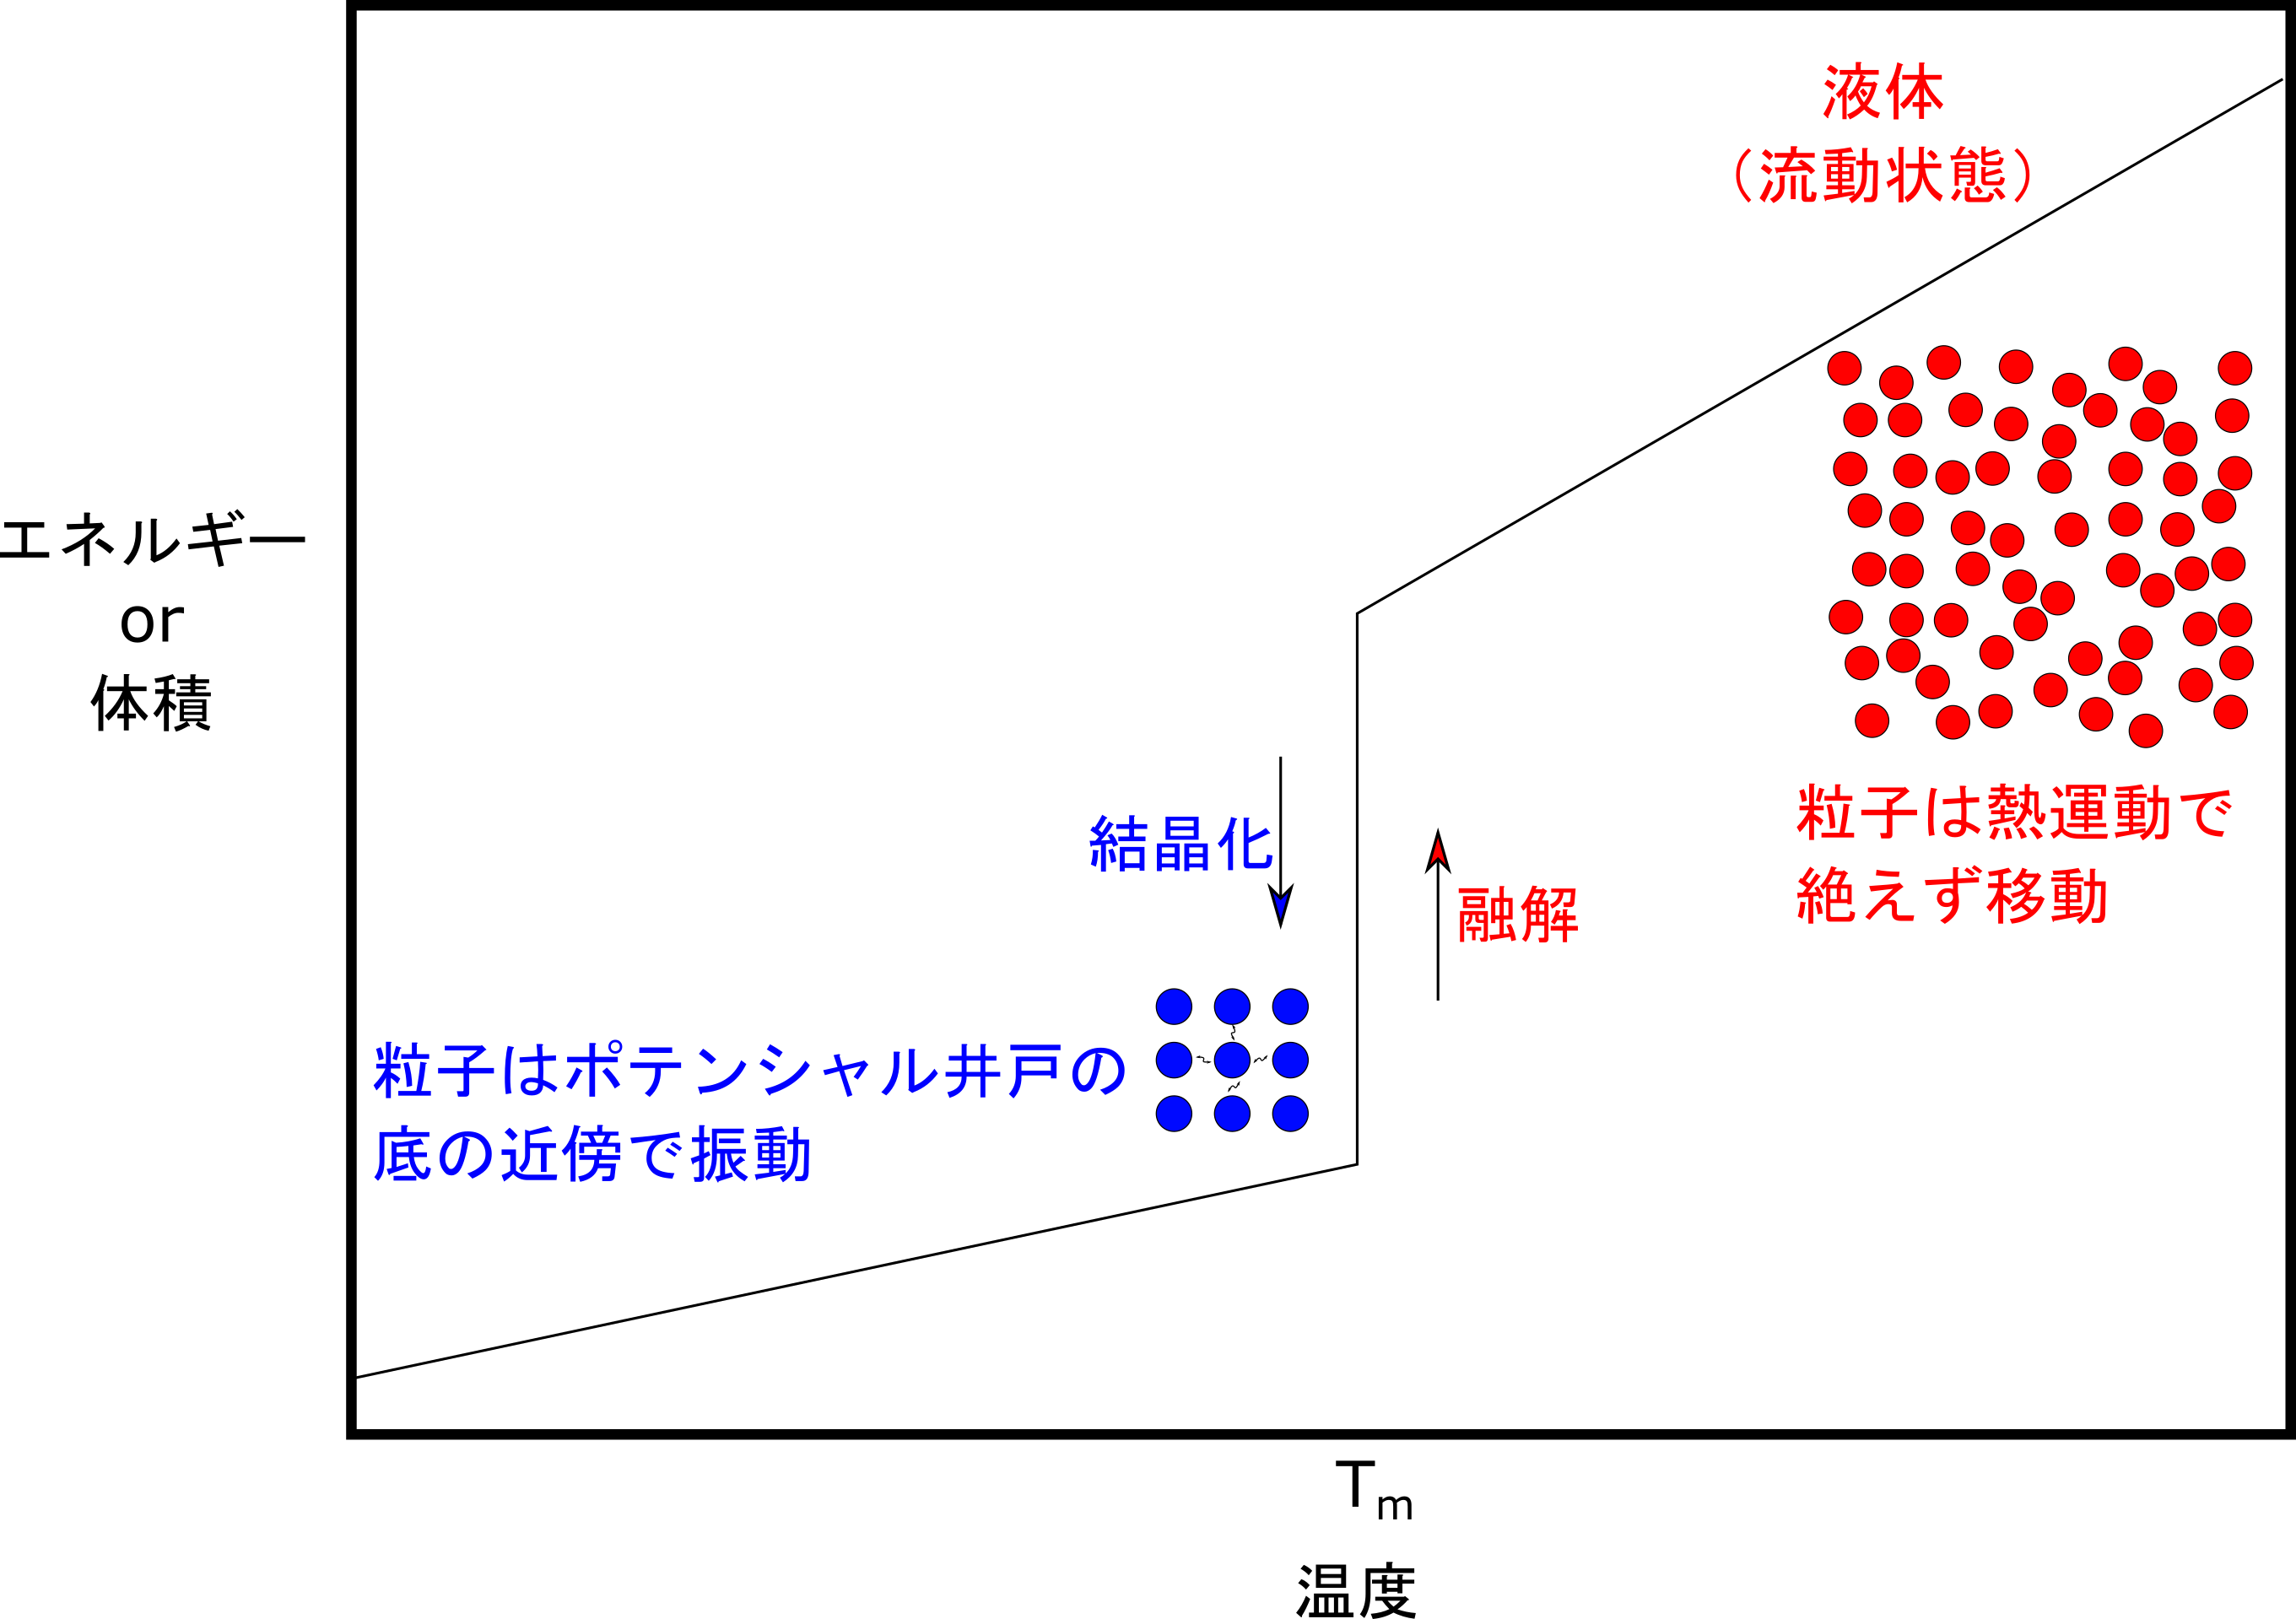
\includegraphics[width=\textwidth]{crystal_melt.png}
			\end{center}
		\end{minipage}
		\caption{固体と液体の相転移}
		\label{fig:crystal_melt}
	\end{center}
\end{figure}

この相転移現象に基づく粒子の振る舞いの変化を、分子動力学シミュレーションで見てみましょう。

図 \ref{fig:MD-kotai} に示した固体\index{こたい@固体}のシミュレーションと同じ初期構造のものを、シミュレーション温度を高温に(T=1.0)した場合です。
図の下に示したリンクをクリックすれば、動画を見ることができます\footnote{
	紙ベースでは、\url{https://drive.google.com/file/d/1ceUaJomvBvljykBGIyLaRJXQbGJzlGUm/view?usp=sharing}
}。
粒子が固体状態での規則構造にとどまることなく、自由に運動していることが確認できます。

温度の上昇により、粒子\index{りゅうし@粒子}の運動が激化して安定位置から脱出しています。
固体状態の規則的な構造が乱れていますので、粒子間の距離も伸びているようですが、このスナップショットからはそこまではわかりません。
\begin{figure}[htb]
	\begin{center}
		\begin{minipage}{0.4\textwidth}
			\large
			\begin{itembox}[l]{分子動力学シミュレーション}
				\begin{itemize}
					\item 温度を高温に(T=1.0)
					\item 粒子の運動が激化
					\item 安定位置から脱出
					\item 粒子間の距離が伸びる
				\end{itemize}
			\end{itembox}
		\end{minipage}
		\begin{minipage}{0.5\textwidth}
			\begin{center}
				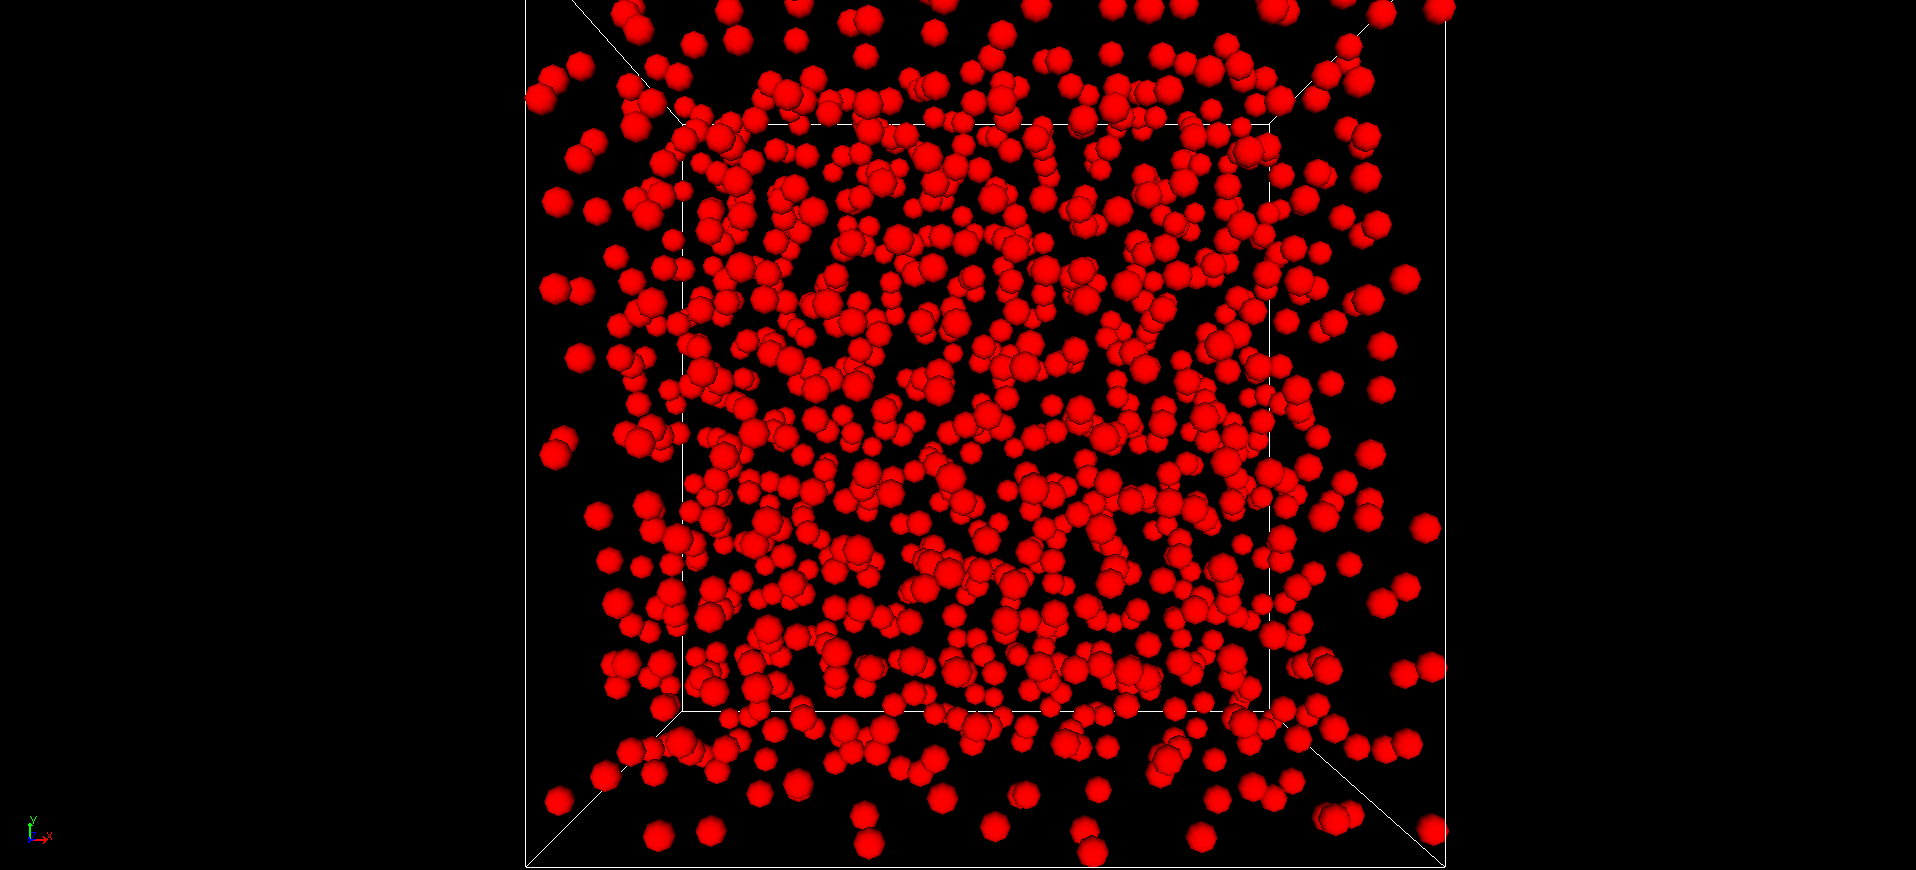
\includegraphics[width=\textwidth]{N1_Melt.png}

				\href{https://drive.google.com/file/d/1ceUaJomvBvljykBGIyLaRJXQbGJzlGUm/view?usp=sharing}{\textcolor{red}{動画へのリンク}}
			\end{center}
		\end{minipage}
		\caption{分子動力学シミュレーションで見た液体}
		\label{fig:MD-ekitai}
	\end{center}
\end{figure}

\subsubsection{粒子間の状態を観る}
次に、粒子同士の相互の位置関係、すなわち、並び具合を評価する方法について簡単に説明します。

物質が粒子から成り立っている場合、「動径分布\index{どうけいぶんぷ@動径分布}関数」という考え方に基づいて、内部の粒子\index{りゅうし@粒子}の状態を評価することができます。
これは、以下のような手順となっていて、一つの粒子から見た場合の他の粒子\index{りゅうし@粒子}の存在比率を粒子間の距離の関数\index{かんすう@関数}として表すことができます\footnote{
	この方法は、シミュレーションだけで行われているのではなく、実験においても散乱関数\index{さんらんかんすう@散乱関数}という X 線や中性子線を物質に照射して
	内部の微細な構造を測定する場合にも使われています。
}。
\begin{itemize}
	\item まず、任意の粒子に着目して、
	\begin{itemize}
		\item 距離の関数として、
		\item 他粒子を数えあげる。
	\end{itemize}
	\item すべての粒子で、同じことをやる。
\end{itemize}

図 \ref{fig:gr} に、動径分布\index{どうけいぶんぷ@動径分布}関数の原理とその例を示しました。

動径分布関数で比べた場合、固体\index{こたい@固体}の動径分布では細かいピークが立ち、その最低値は 0 に近くなっていて、
それが遠くの位置にまで連なっていることが見て取れます。
このピークの存在と最低値が 0 近くに下がっていることは、特定の位置における粒子の存在が偏在化していて、
その間においては粒子\index{りゅうし@粒子}が存在しない領域があることを示しており、また、そのような構造が遠距離にまで連続していることを示しています。
\begin{figure}[htb]
	\begin{center}
		\begin{minipage}{0.4\textwidth}
			\large
			\begin{itembox}[l]{動径分布\index{どうけいぶんぷ@動径分布}関数とは、}
				\begin{itemize}
					\item ある粒子からみて、距離の関数として球殻上の他粒子を数えあげる。
					\item すべての粒子で、同じことをやる。
				\end{itemize}
			\end{itembox}
			\begin{center}
				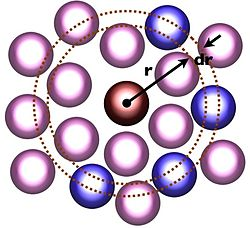
\includegraphics[width=.9\textwidth]{gr.jpg}
				\end{center}
		\end{minipage}
		\begin{minipage}{0.5\textwidth}
			\large
			\begin{itembox}[l]{シミュレーションの動径分布関数}
				\begin{itemize}
					\item 固体の動径分布関数
					
					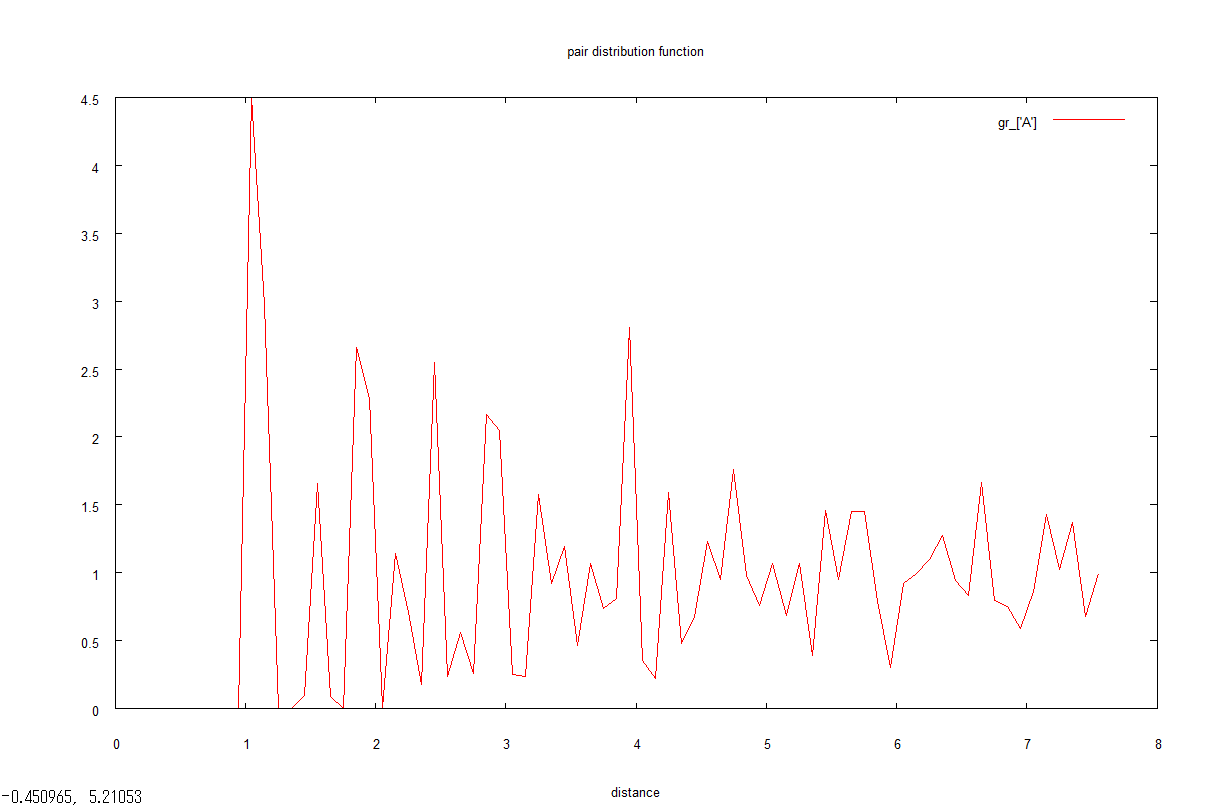
\includegraphics[width=.8\textwidth]{Gr_N1_Cry_T_0_1.png}
					\item 液体の動径分布関数
					
					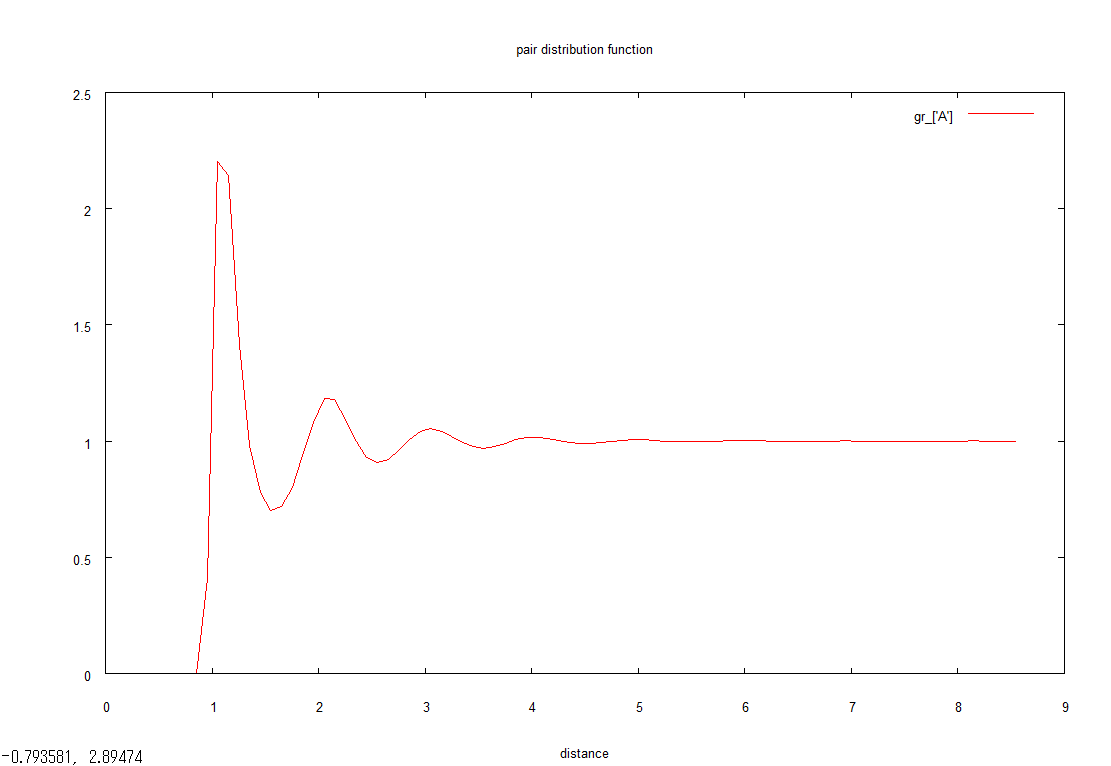
\includegraphics[width=.8\textwidth]{Gr_N1_Cry_T_1.png}
				\end{itemize}
			\end{itembox}
		\end{minipage}
		\caption{動径分布関数で観る固体と液体}
		\label{fig:gr}
	\end{center}
\end{figure}

一方、液体\index{えきたい@液体}の動径分布においては、最も近接したピークとその隣のピークぐらいははっきりと見えますが、
それよりも遠距離では見えなくなっています。
また、最低値も固体\index{こたい@固体}と比較すれば遥かに高いものであることがわかります。
この液体\index{えきたい@液体}での動径分布関数の振る舞いは、液体の中では粒子\index{りゅうし@粒子}の相互作用\index{そうご@相互作用}はたかだか粒子数個分にしか到達しなくて、
全体としてみれば乱雑な状態として均一な関係を持っていることが推定できます。

\subsubsection{液体\index{えきたい@液体}をミクロに観ると}
もう少しだけ、ミクロに見た場合の液体における密度のゆらぎ\footnote{
	「ゆらぎ」という言葉も定義がちょっと難しいのですが、ここでは、場所ごとの密度の高いところと低いところの分布具合とでも捉えてください。
}について考察を進めましょう。
図 \ref{fig:liquid_doukei} に液体の動径分布\index{どうけいぶんぷ@動径分布}関数について、密度との関係から見てみたものを示しました。
\begin{figure}[htb]
	\begin{center}
		\begin{minipage}{0.4\textwidth}
			\large
			\begin{itembox}[l]{液体の局所的な密度}
				\begin{itemize}
					\item 液体の相互の位置は、\\規則的ではない。
					\item 粒子径 (r/$\sigma$=1) よりも、\\少し離れた所にピーク。
					\item それより少し遠くに、\\密度の低い領域が。
				\end{itemize}
			\end{itembox}
		\end{minipage}
		\begin{minipage}{0.5\textwidth}
			\begin{center}
			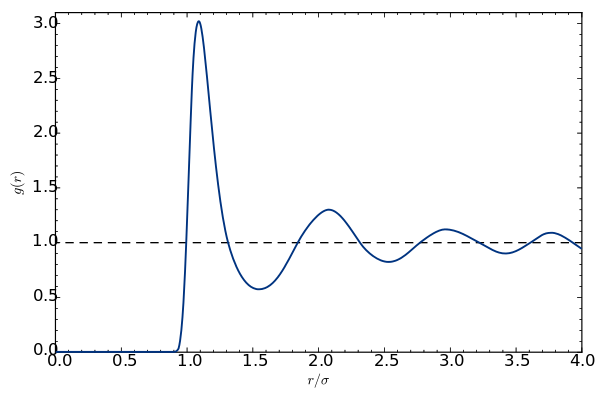
\includegraphics[width=.9\textwidth]{gr_2.png}
			\end{center}
		\end{minipage}
		\caption{液体の局所的な密度}
		\label{fig:liquid_doukei}
	\end{center}
\end{figure}

繰り返しになりますが、液体\index{えきたい@液体}における粒子の相互の位置は規則的ではなく、粒子径 (r/$\sigma$=1) よりも少し離れたところにピークがありそのあたりで若干密度が高いこと、また、それよりも少し遠くでは平均値よりも密度の低い領域が存在しています。

このような液体\index{えきたい@液体}の配列状態において、シミュレーションの動画で確認したように、乱雑に並んだ粒子がそれぞれ異なる方向へと移動しているわけです。
動径分布関数を考慮すると、この移動は、粒子同士の運動の結果として瞬間瞬間に生じている僅かに密度の低い領域に粒子\index{りゅうし@粒子}が移動した結果と考えることができることになります。
これが、粒子\index{りゅうし@粒子}が移動して拡散していく現象のミクロな状態のモデルということになります。
\begin{figure}[htb]
	\begin{center}
		\large
			\begin{minipage}{0.45\textwidth}
				\begin{itembox}[l]{粒子の移動}
					\begin{itemize}
						\item 乱雑に並んだ粒子が、
						\item それぞれ異なる方向へ移動
					\end{itemize}
				\end{itembox}
				\vspace{3mm}
				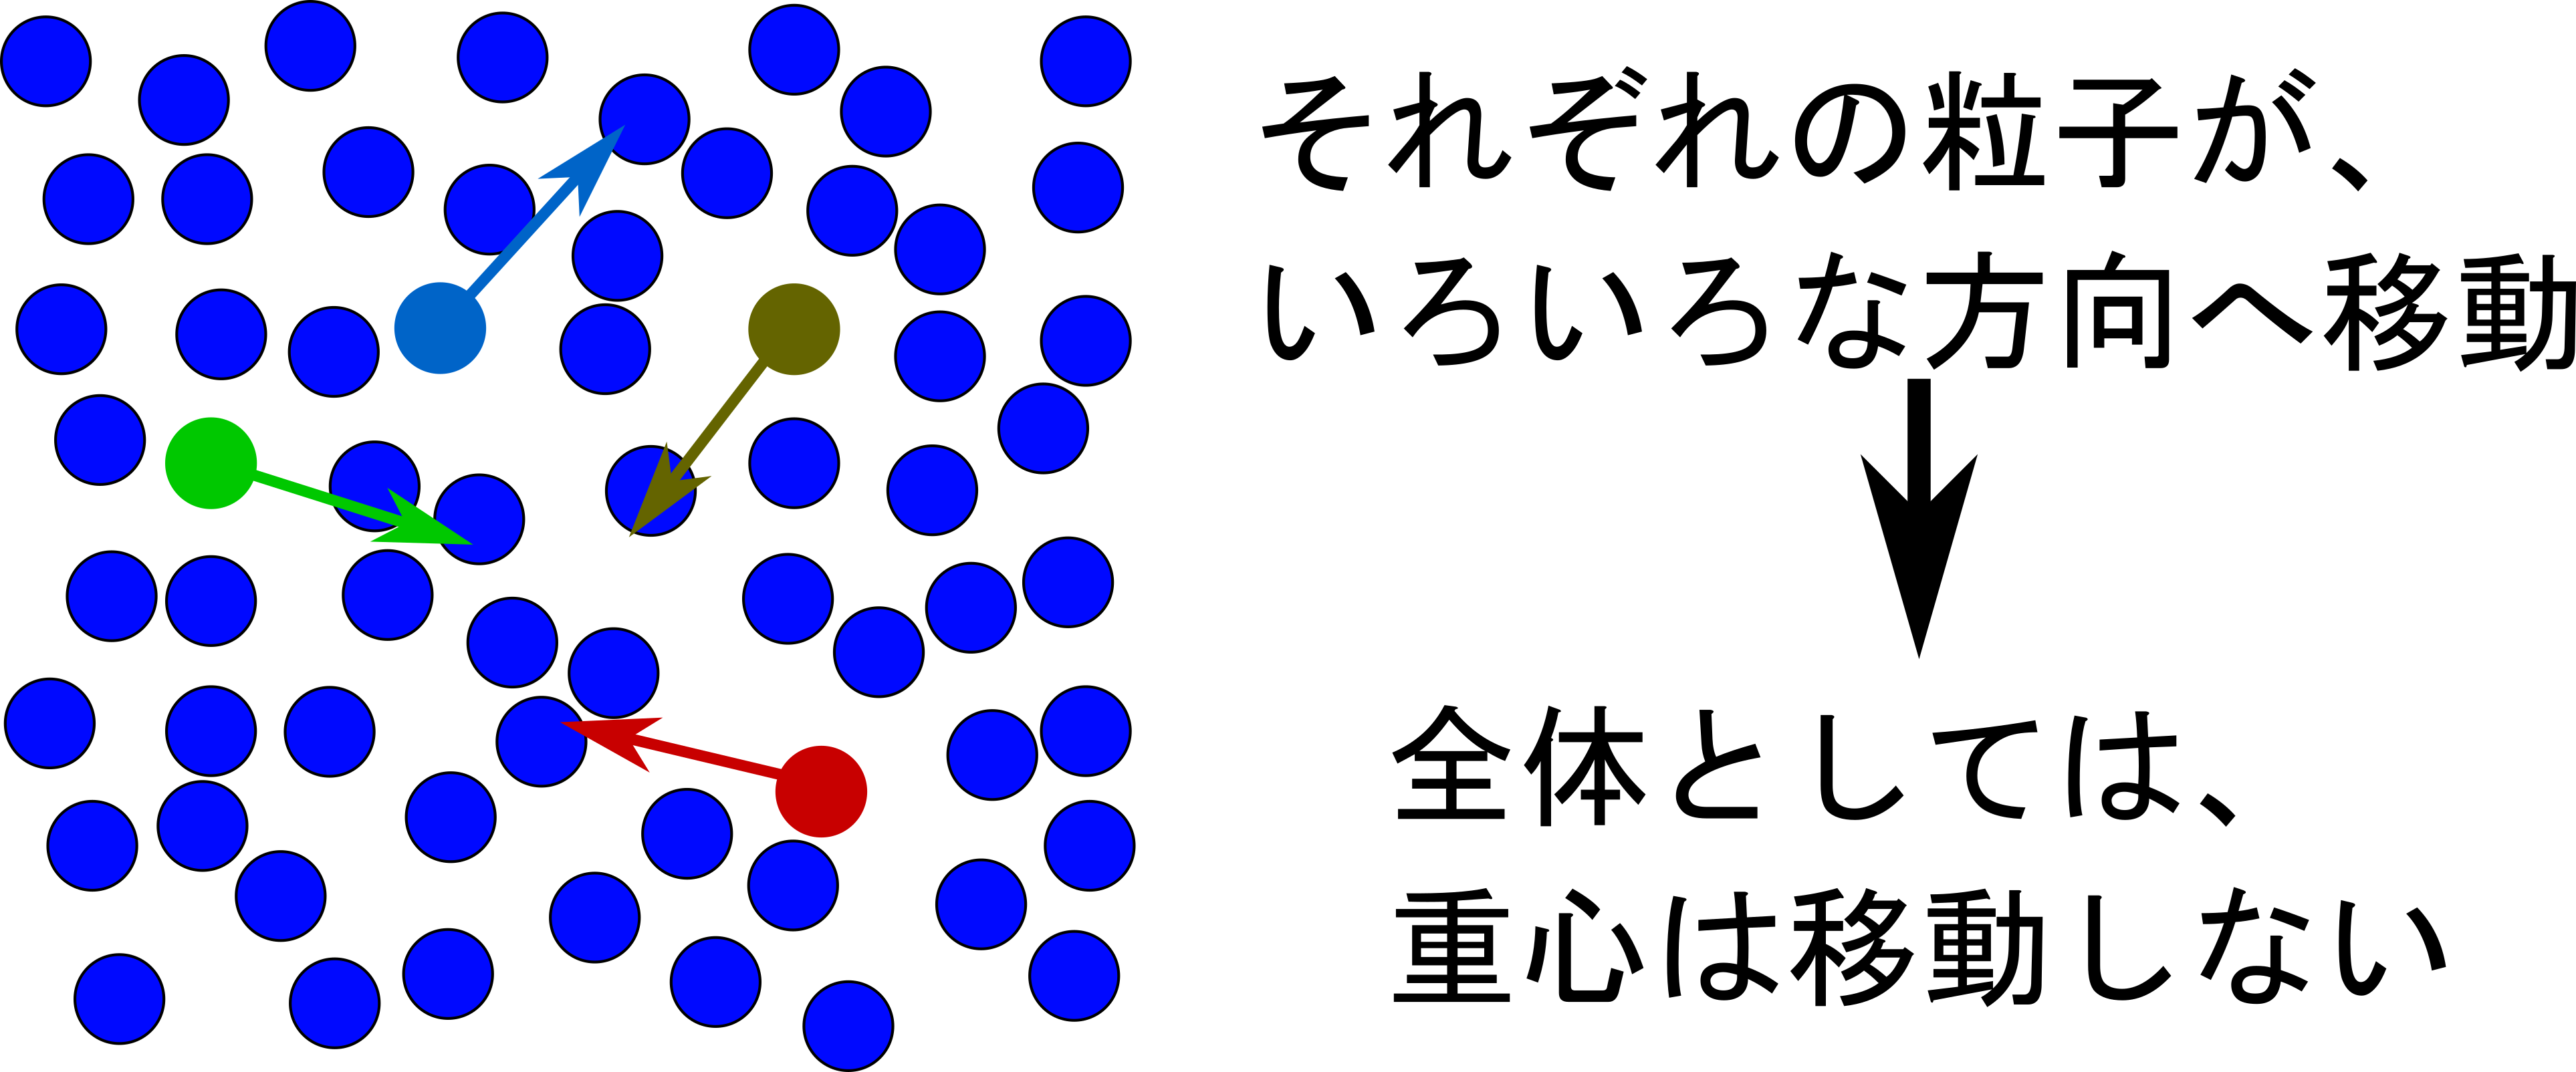
\includegraphics[width=\textwidth]{liquid_model.png}
			\end{minipage}
			\begin{minipage}{0.45\textwidth}
				\begin{itembox}[l]{粒子の拡散}
					\begin{itemize}
						\item 一粒子に着目すると、
						\item 少しずつ元の位置から移動
					\end{itemize}
				\end{itembox}
				\vspace{3mm}
				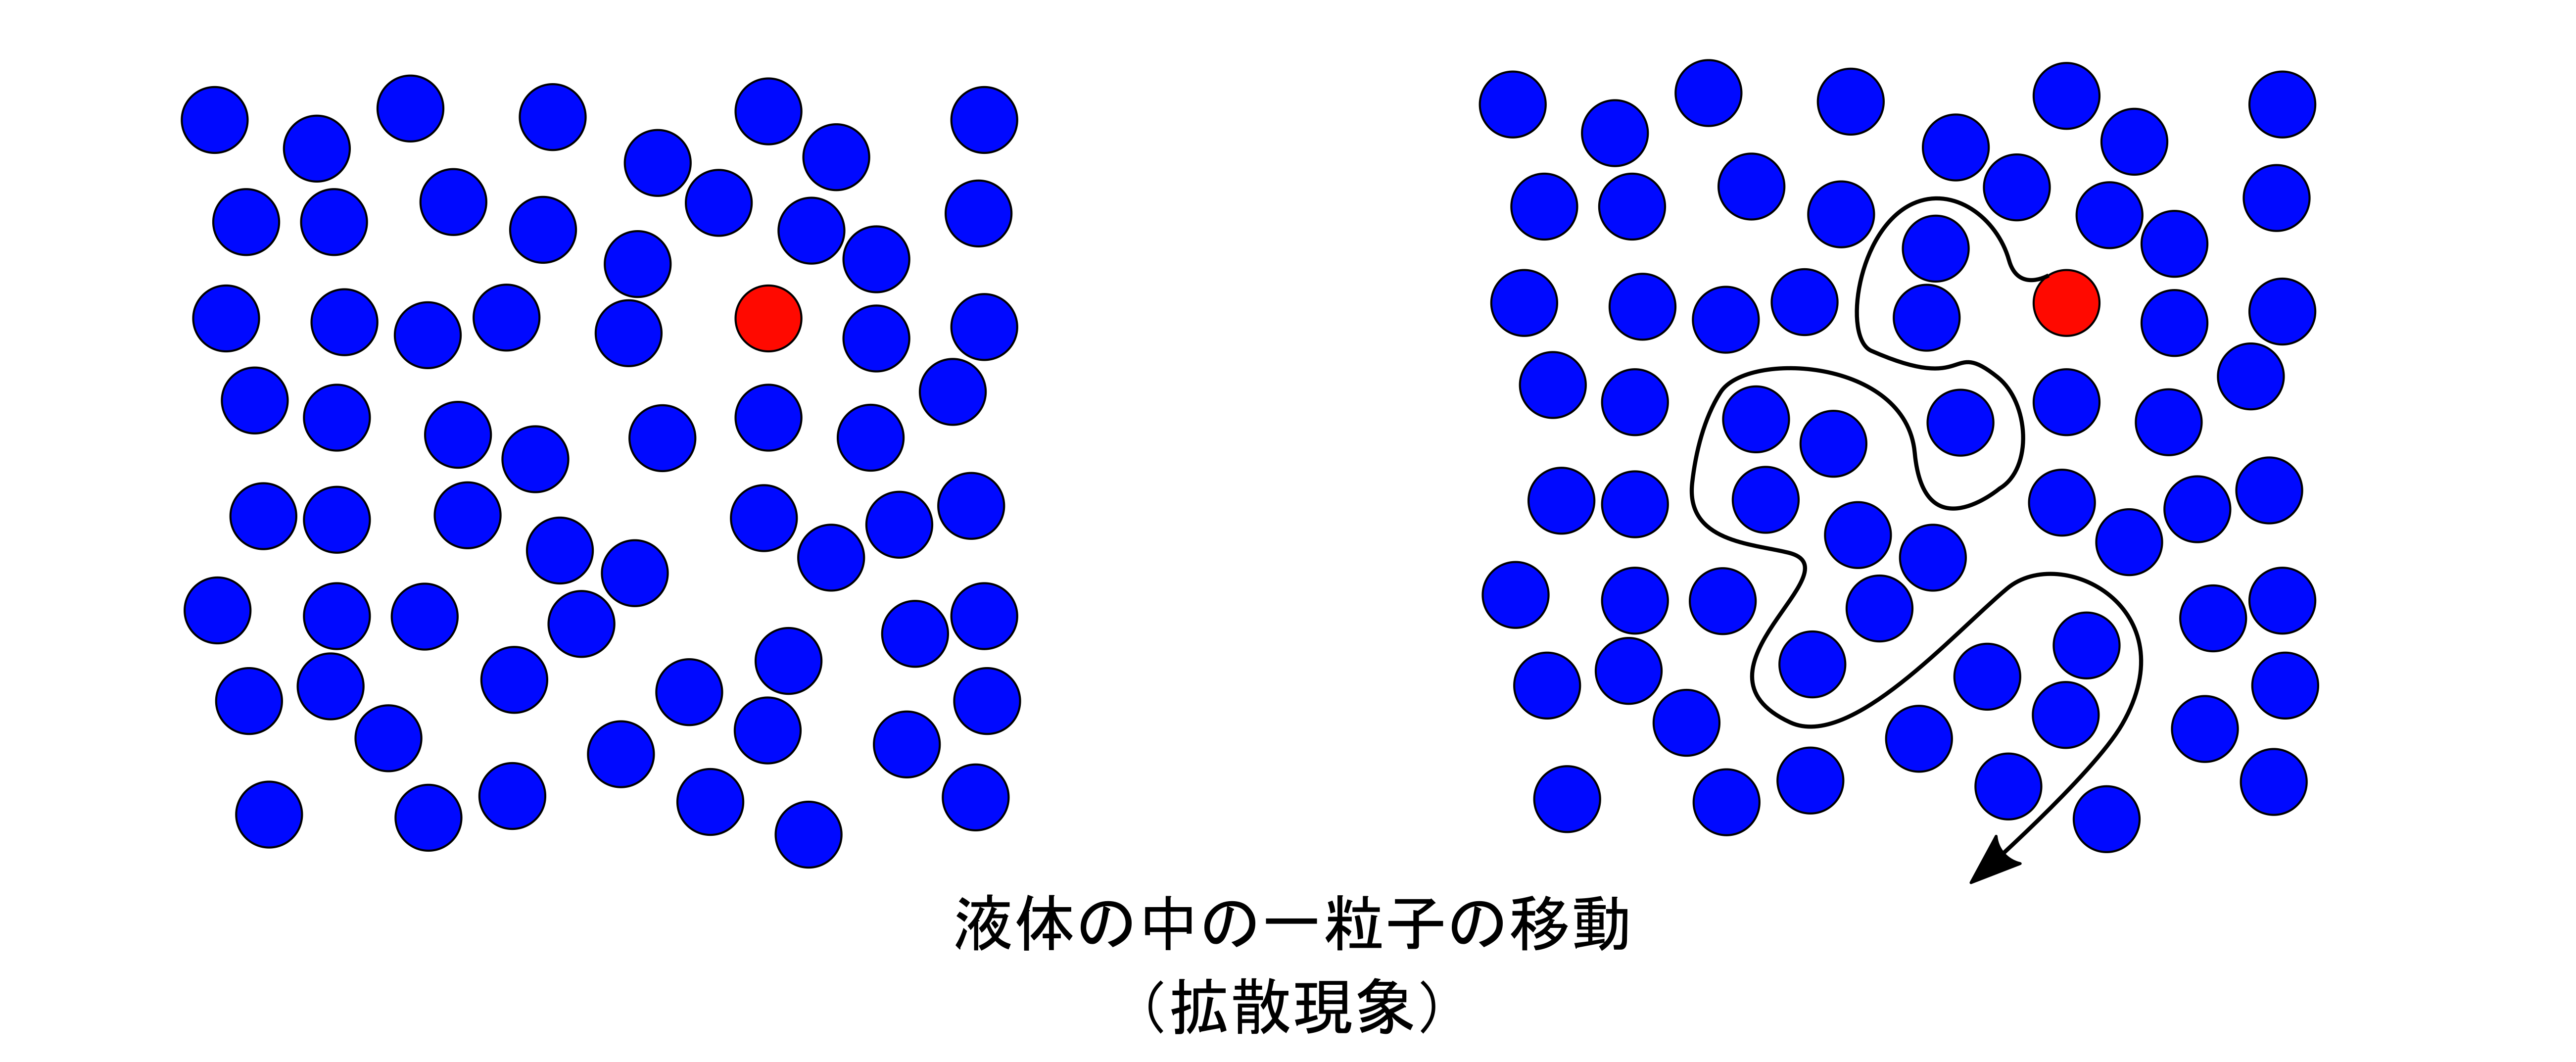
\includegraphics[width=\textwidth]{liquid_1.png}
			\end{minipage}	
		\caption{液体での粒子の移動}
		\label{fig:ekitai_idou}
	\end{center}
\end{figure}

注意していただきたいのは、例えばコップに入った水のように周りを拘束された状態では水は止まって見えているということです。
そのような状態においても、ミクロに見れば、粒子\index{りゅうし@粒子}は絶えず移動して入れ替わっています。
しかしながら、それぞれの粒子\index{りゅうし@粒子}の移動方向がてんでバラバラ(等方的)になっていて、その結果として、全体の重心は移動しないわけです。

このミクロな運動のことを意識していただければ、次の節での「流れる」ということの理解が容易になります。
\begin{figure}[htb]
	\begin{center}
		\begin{minipage}{0.55\textwidth}
			\large
			\begin{itembox}[l]{コップの中の水}
				\begin{itemize}
					\item マクロには、
					\begin{itemize}
						\item 変化しない:止まって見える
					\end{itemize}
					\item ミクロには、
					\begin{itemize}
						\item 熱エネルギーで粒子がランダム運動
						\item 粒子の近くに隙間ができると移動
						\item その移動により別の隙間ができ、\\他の粒子がそこに移動。
						\item 上記の相互の入れ替えは、常に発生。
					\end{itemize}
				\end{itemize}
			\end{itembox}
		\end{minipage}
		\begin{minipage}{0.35\textwidth}
			\begin{center}
			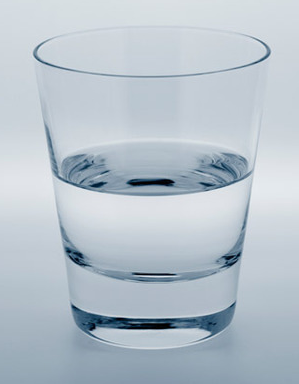
\includegraphics[width=.8\textwidth]{cup_water.png}
			% \vspace{5mm}
			% 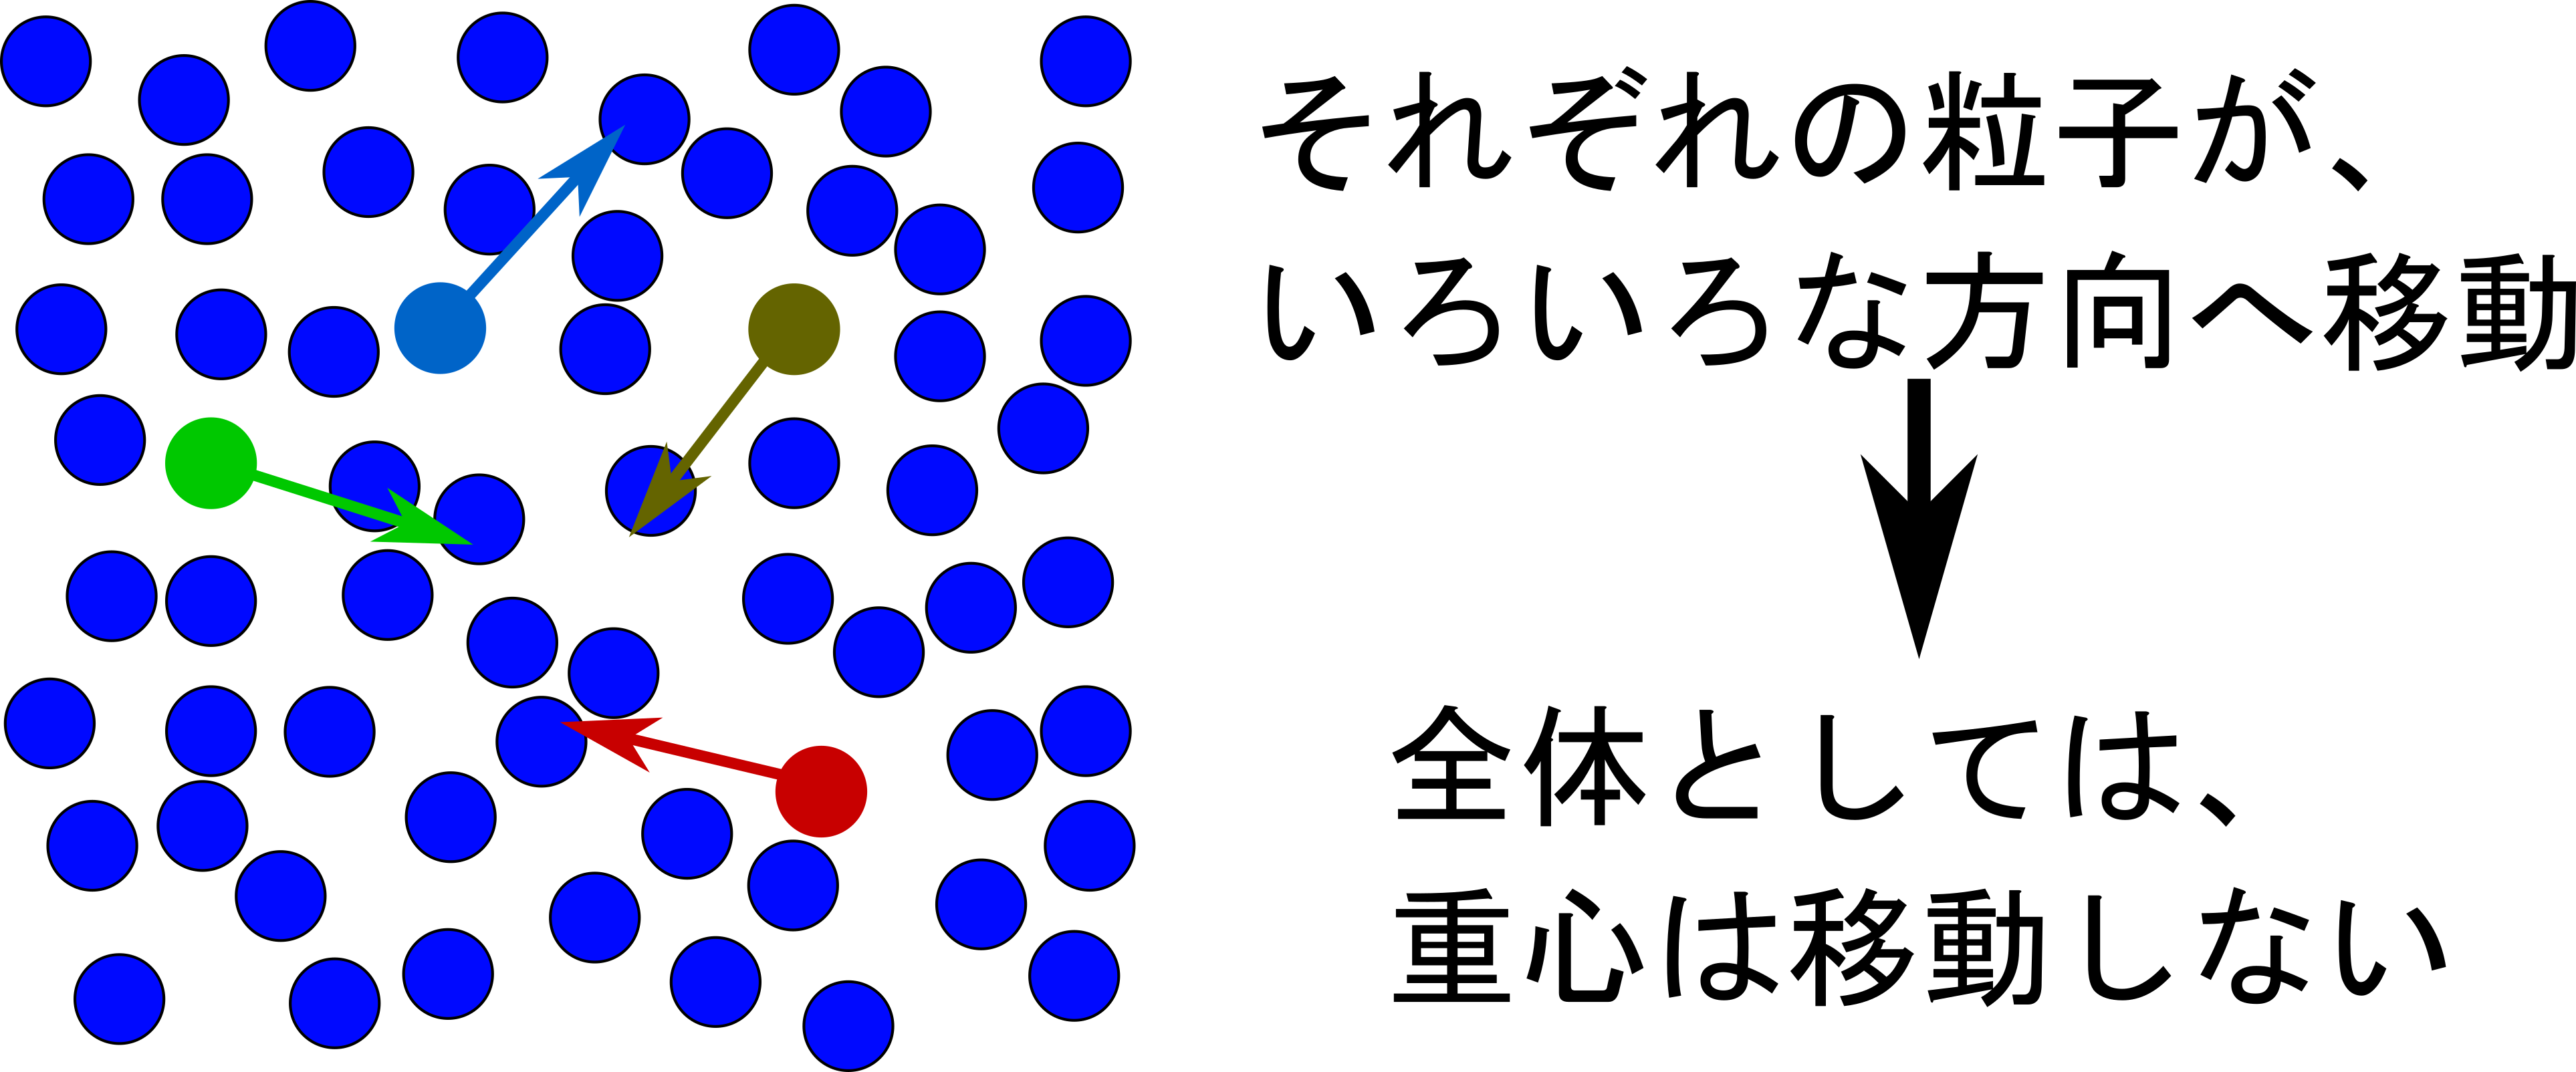
\includegraphics[width=.9\textwidth]{liquid_model.png}
			\end{center}
		\end{minipage}
		\caption{コップの中の水について考えてみると}
		\label{}
	\end{center}
\end{figure}

\subsubsection{固体\index{こたい@固体}と液体\index{えきたい@液体}}

ここまで、ミクロに捉えた粒子描像として見た場合の固体\index{こたい@固体}と液体\index{えきたい@液体}の違いについて、説明してきました。

この節のまとめとして、固体\index{こたい@固体}と液体の違いについて、簡単にまとめましょう。
まず、物質の三態をミクロに捉えて、雰囲気温度での粒子\index{りゅうし@粒子}の運動を考えると、以下のように考えることができます。
\begin{figure}[htb]
	\begin{center}
		\begin{minipage}{0.48\textwidth}
			\large
			\begin{itembox}[l]{温度ベースで考えると、}
				\begin{itemize}
					\item 高温では気体:粒子が自由に移動
					\item 中温では液体:適度に移動できる
					\item 低温では固体:\\
					落ち着きのいい位置に留まる
				\end{itemize}
			\end{itembox}
		\end{minipage}
		\begin{minipage}{0.42\textwidth}
			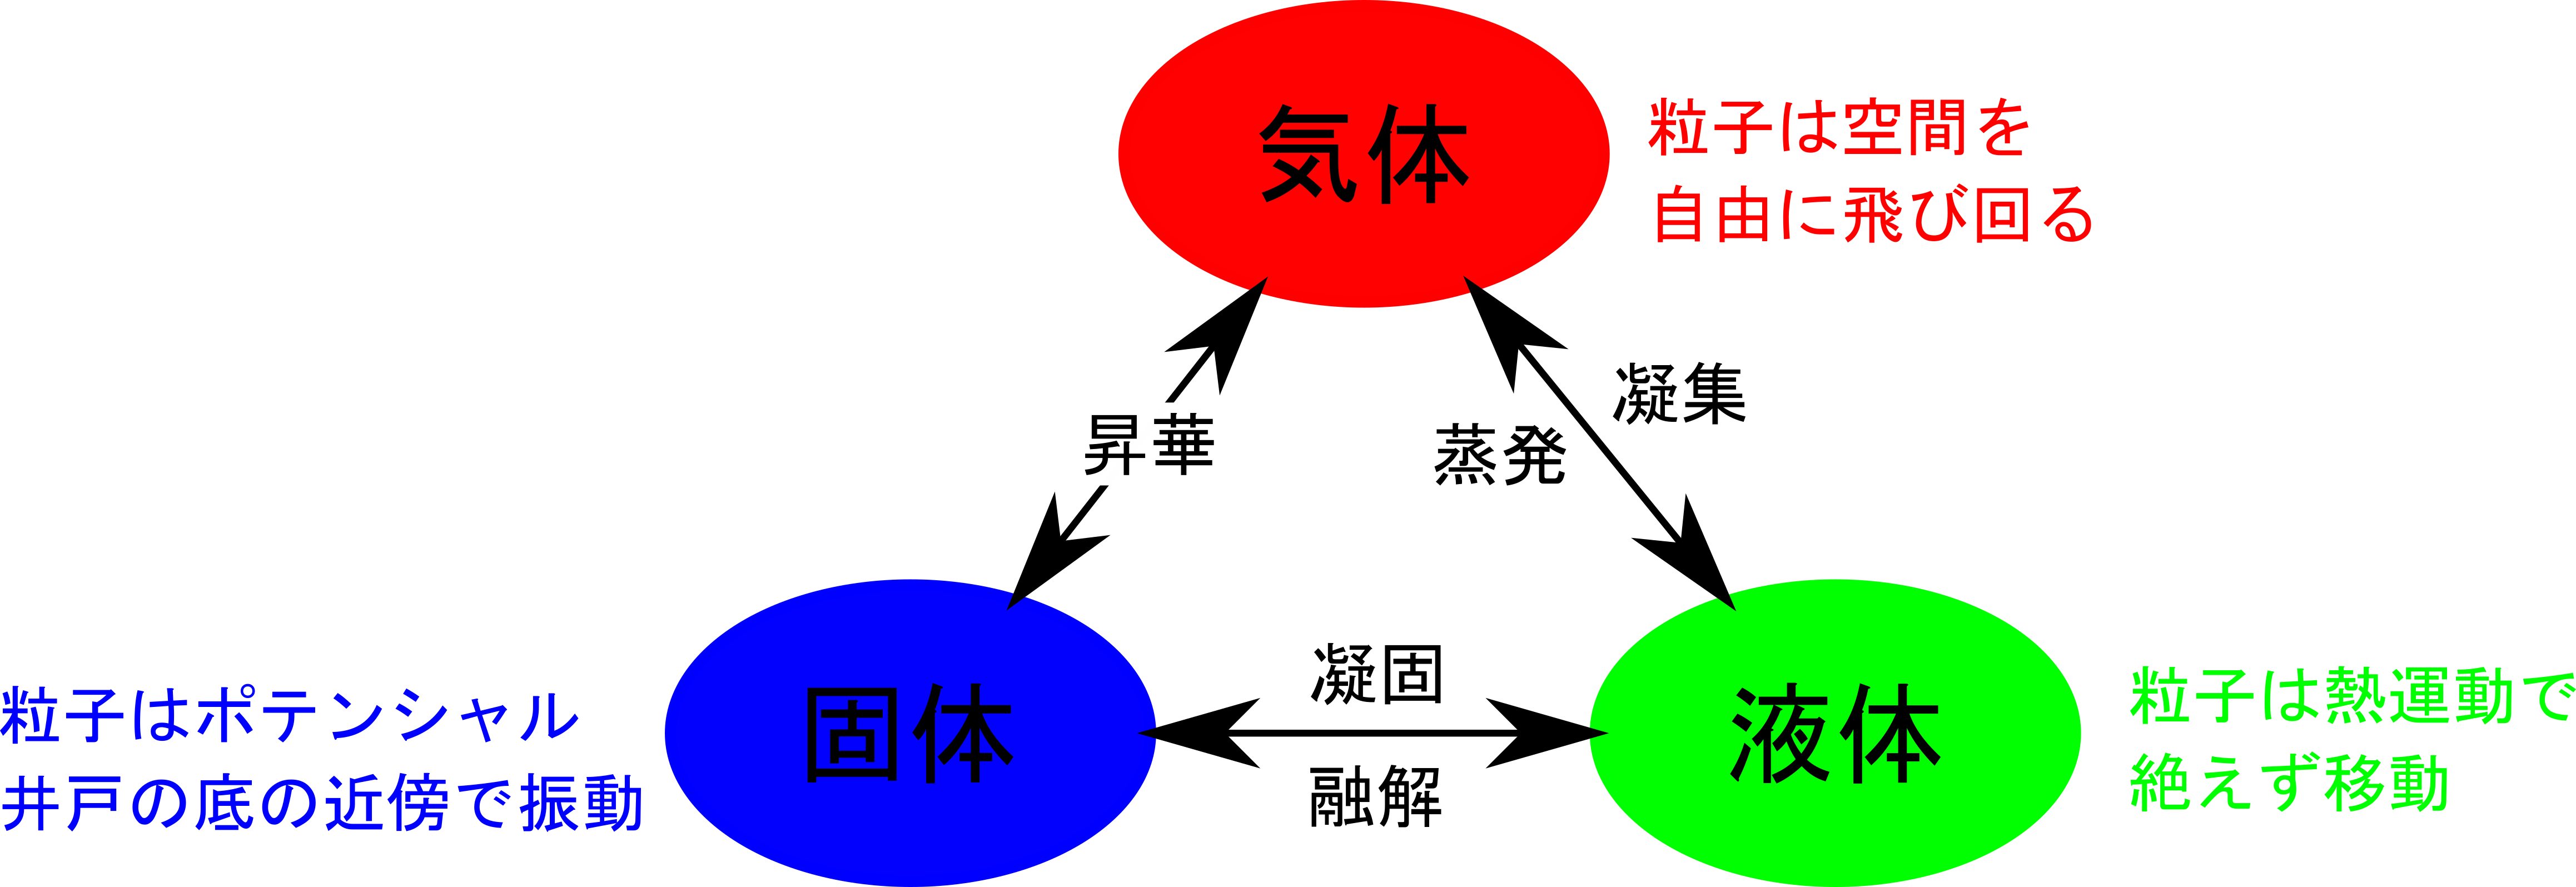
\includegraphics[width=\textwidth]{3Phase.png}
		\end{minipage}
		\caption{物質の三態をミクロに捉えると}
		\label{fig:santai_micro}
	\end{center}
\end{figure}

もう少し細かく、ミクロな粒子の振る舞いを考えれば、熱エネルギーにより揺らされて自由に動こうとするという状態と、ポテンシャル\index{ぽてんしゃる@ポテンシャル}井戸の底の居心地のいい位置に留まりたいという状態との、2つの状態のせめぎあいであると考えることができます。
雰囲気温度に応じて、このどちらかの状態の一方が優勢となって、マクロな状態を決めているのです。

\large
\begin{itembox}[l]{ミクロに考えた固体と液体の違い}
	\begin{itembox}[l]{ミクロな状態での2つのせめぎあい}
		\begin{itemize}
			\item 粒子は熱エネルギーで揺らされる。
			\item 居心地のいい位置に留まりたい。
		\end{itemize}
	\end{itembox}
	\begin{itembox}[l]{その結果として、}
		\begin{itemize}
			\item 固体:相対的に揺動小
			\begin{itemize}
				\item ポテンシャル井戸の底近傍で振動
				\item 内部構造を形成。
			\end{itemize}
			\item 液体:熱揺動が大きい
			\begin{itemize}
				\item 多くの粒子が相互作用
				\item 構造が不定
			\end{itemize}
		\end{itemize}
	\end{itembox}
\end{itembox}
\normalsize

\section{流れるということは?}

さて、これでようやく準備が整ってきましたので、レオロジーを考える場合に最も重要な事項である「流れる」ということについての考察へと入っていきましょう。

\subsection{マクロな変形と粒子の移動}

まず、流れるということをマクロに考えてみましょう。

コップの中の水は流れませんでした。
これは、水がコップという形状によって拘束されているから、その位置に留まっているものと考えることができます。
すなわち、ものが流れるということは、そのような拘束を解いてマクロな変形を与えることによって流れると言えます。
具体的には、コップを傾けてやれば水はコップの中を流れて移動しますし、もっと傾ければコップから流れ出していきます。

これをミクロな粒子の絵として考えてみましょう。
マクロな変形が付与されたとき、ミクロに見たときの粒子\index{りゅうし@粒子}の相互の位置も変化します。
このとき、粒子同士の多体としてのポテンシャルも変化して、部分的に居心地の悪い粒子が発生します。
もともと、マクロな変形がなければ、粒子\index{りゅうし@粒子}の運動は等方的にどちらへも均等に移動しようとしていましたが、このポテンシャルの変化により移動のバランスが変化して、それぞれの粒子\index{りゅうし@粒子}が居心地のいい位置へと再配置していくようになります。
それらのミクロな移動の結果として、マクロな変形に従うようにミクロな粒子の位置が最適化していくことになります。
\begin{figure}[htb]
	\begin{center}
		\begin{minipage}{0.5\textwidth}
			\large
			\begin{itembox}[l]{ミクロな流動のイメージ}
				\begin{itemize}
					\item マクロな変形を与える。
					\begin{itemize}
						\item ミクロに粒子の相互位置が変化
						\item 相互のポテンシャルのために、\\居心地が悪い粒子が発生。
						\item 粒子の移動のバランスが変化
						\item 居心地のいい位置へと再配置
					\end{itemize}
					\item マクロな変形に従うように、粒子の位置が最適化。
				\end{itemize}
			\end{itembox}
		\end{minipage}
		\begin{minipage}{0.4\textwidth}
			\begin{center}
			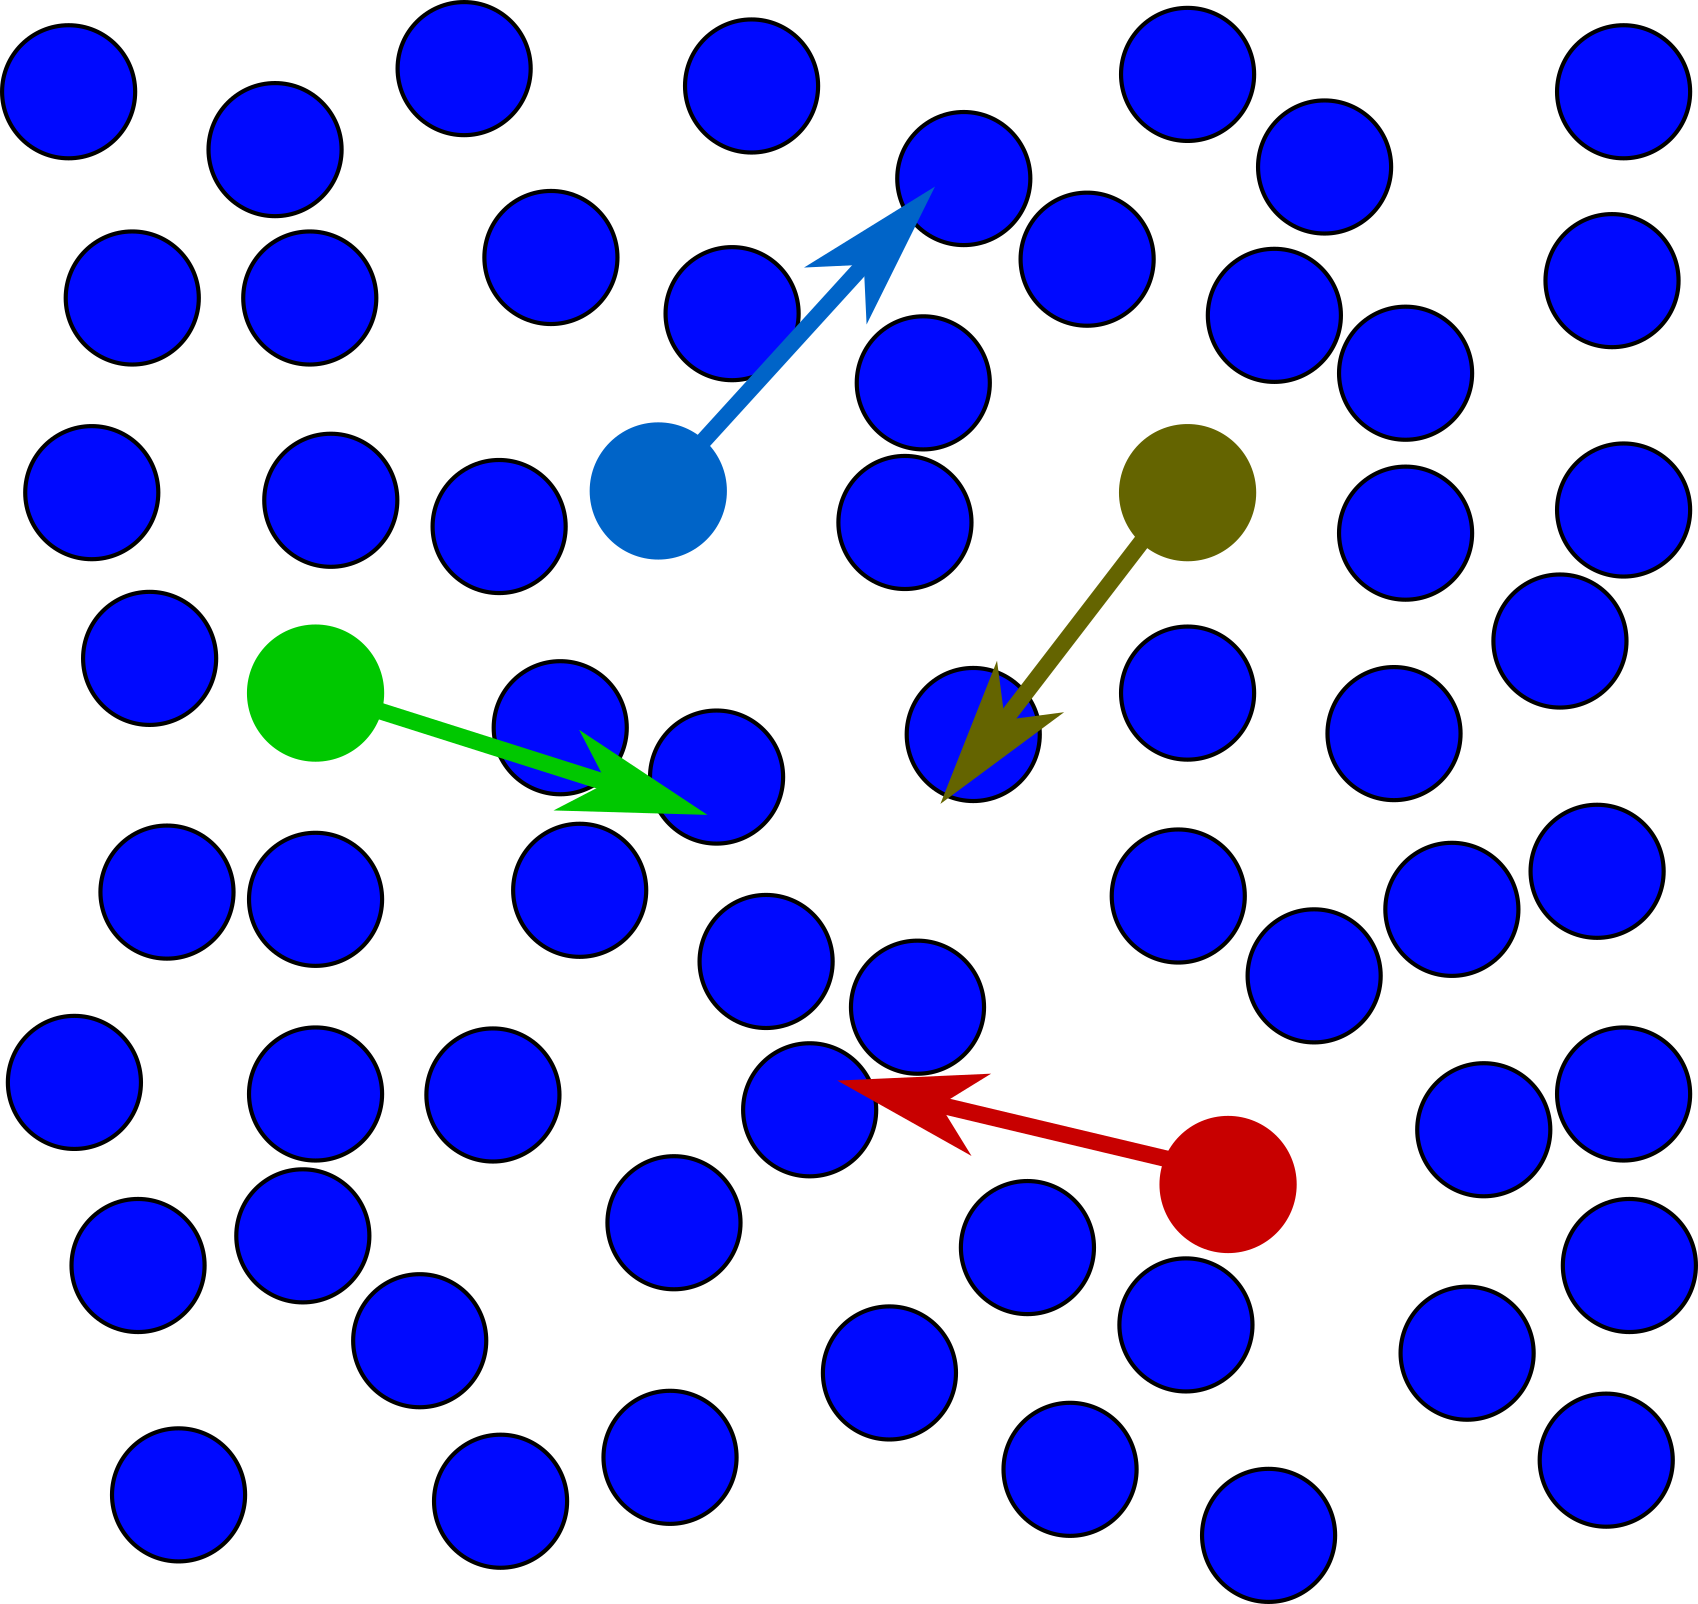
\includegraphics[width=.9\textwidth]{liquid_model_2.png}
			\end{center}
		\end{minipage}
		\caption{ミクロな流動のイメージ}
		\label{fig:micro_ryuudou}
	\end{center}
\end{figure}

\subsection{固体\index{こたい@固体}と液体\index{えきたい@液体}の境目を時間で考えると}

流れるということのミクロな描像も少しずつイメージできてきました。

次に、時間の因子を考えながら、固体\index{こたい@固体}と液体\index{えきたい@液体}の境目について考えてみましょう。

\subsubsection{速い変形を考えた場合}

液体\index{えきたい@液体}が流動するということをミクロに考えると、粒子間の密度ゆらぎの結果として瞬間的に生じる隙間に粒子\index{りゅうし@粒子}が移動し、その結果として空いた場所に他の粒子\index{りゅうし@粒子}が移動してくるのでした。

では、ミクロに粒子\index{りゅうし@粒子}が動くよりも早くマクロに変形しようとするとどうなるでしょうか。

我々の身近な事象として思い出せば、とても速い速度で水を変形した場合であり、例えば、高い場所から水に飛び込むようなことです。
このとき、水がまるで固体\index{こたい@固体}になったかのようにとても硬いものとして振る舞うことはご存知かと思います。
つまり、「速い変形に対しては、液体\index{えきたい@液体}が固体的に」なるわけです。
\begin{figure}[htb]
	\begin{center}
		\begin{minipage}{0.44\textwidth}
			\begin{center}
			\large
			\begin{itembox}[l]{速い変形では固体的に}
				\begin{itemize}
					\item 流動するとは、
					\begin{itemize}
						\item 隙間に粒子が移動
						\item 空いた場所に他の粒子が移動
					\end{itemize}
					\item 粒子が動くより早く変形しようとすると?
					\begin{itemize}
						\item 速い速度で水を変形\\(高所から飛び込み)
						\item 液体が固体的な挙動
					\end{itemize}
				\end{itemize}
			\end{itembox}
			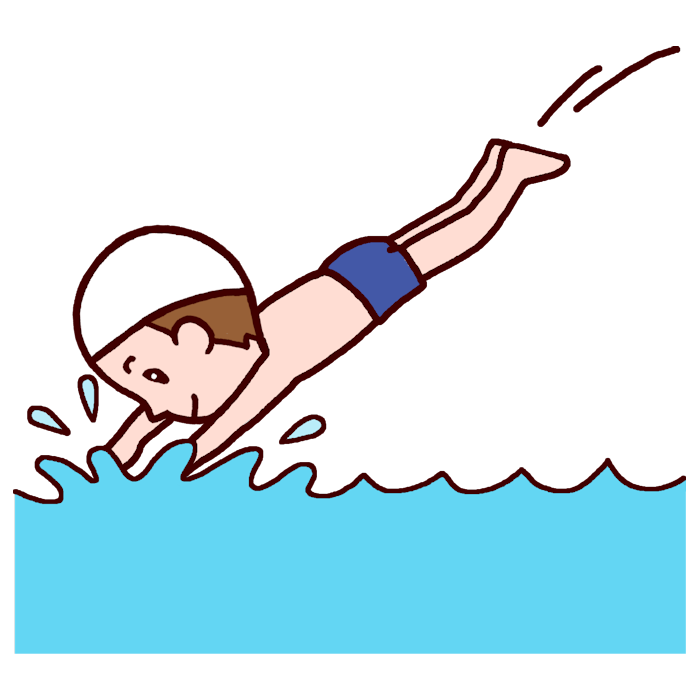
\includegraphics[width=.35\textwidth]{dive.png}
			\end{center}
		\end{minipage}
		\begin{minipage}{0.46\textwidth}
			\begin{center}
			\large
			\begin{itembox}[l]{長時間では液体的に}
				\begin{itemize}
					\item 長時間では氷河も流れる
					
					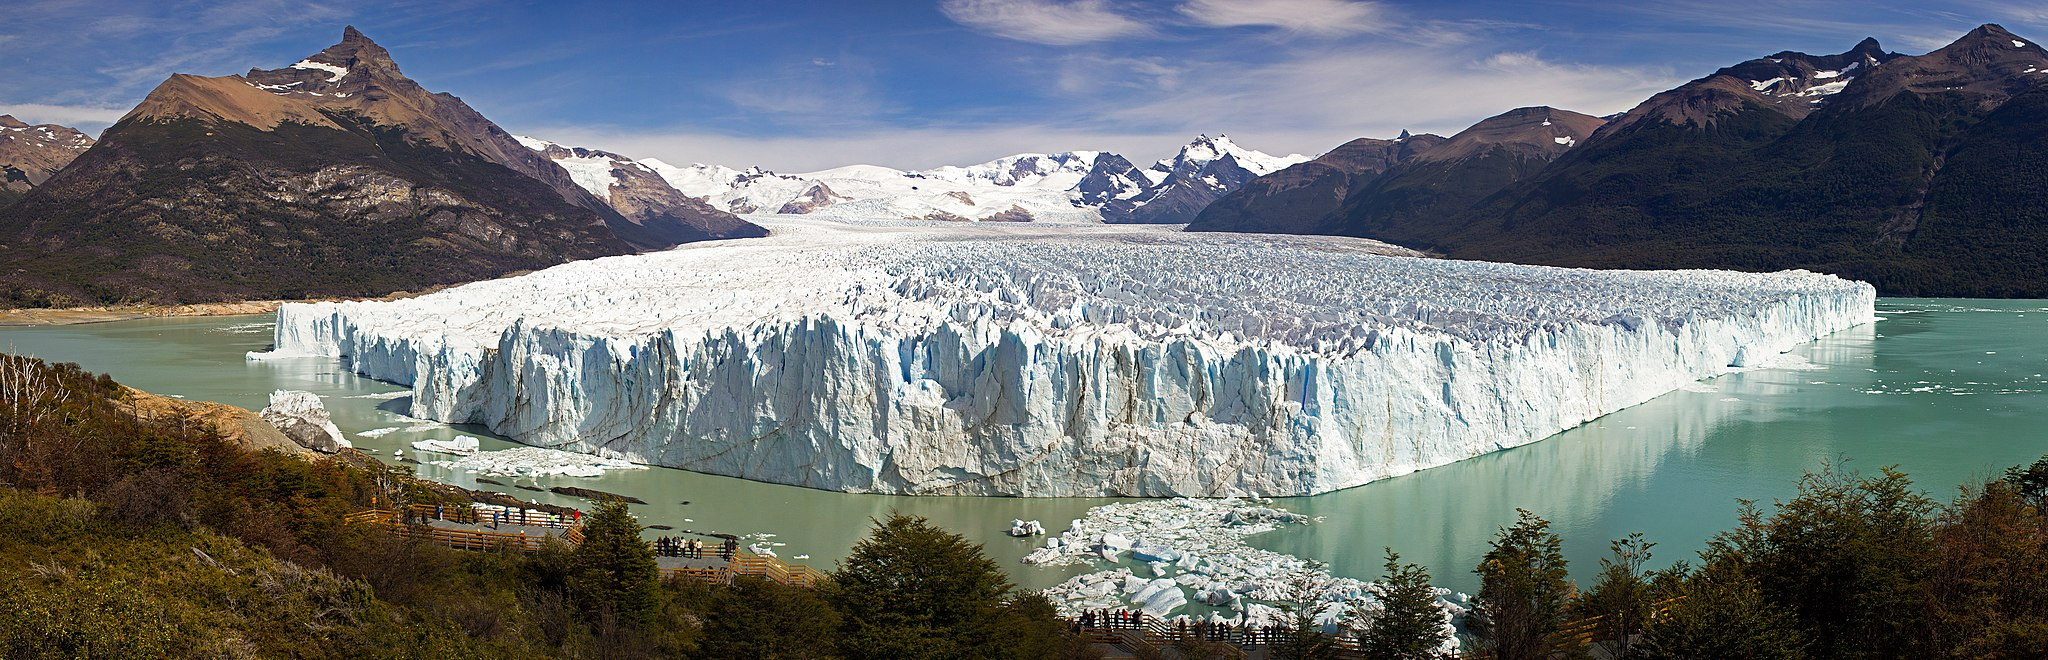
\includegraphics[width=.9\textwidth]{hyoga.jpg}
					\item コールタールも漏斗から\\流れ落ちる	
					
					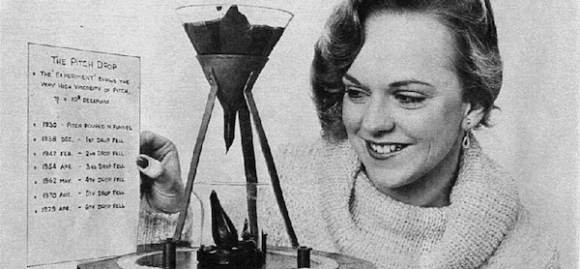
\includegraphics[width=.9\textwidth]{pitchdrop.png}
				\end{itemize}

				\href{https://livestream.com/accounts/4931571/events/5369913}
				{ピッチドロップ実験のライブ画像\\へのリンク}
			\end{itembox}
			\end{center}
		\end{minipage}
		\caption{時間で見た固体と液体の境目は?}
		\label{fig:kotai_ekitai}
	\end{center}
\end{figure}

\subsubsection{長時間に渡る変形では}
つぎに、長時間にわたる変形を考えます。
このとき、経験則として、固体\index{こたい@固体}に見えるものも流れる場合があることを知っているはずです。
例えば、氷河であったり、山であったり、コールタールの場合に見られる現象です。
標語的には、「長時間にわたる変形では、固体\index{こたい@固体}も液体\index{えきたい@液体}的に」なるということです。

この長時間変形で固体\index{こたい@固体}が流れるという現象は、ここまで考えてきた単純な結晶のモデルでは理解しにくいのですが、次に示す「ガラス状態」ということを考えれば、イメージできるようになってきます。

\subsubsection{結局、固体と液体の境目は?}
これら2つの振る舞いをまとめると図 \ref{fig:kotai_ekitai}のようになるわけです。

したがって、時間という因子を明確に定義しないと、固体\index{こたい@固体}と液体\index{えきたい@液体}の境目というのはいささか曖昧になってしまうことが理解できると思います。

\subsection{ガラス状態}

実際の物質においては、液体\index{えきたい@液体}からの冷却によって常に結晶化するとは限りません。
よく知られた例が、窓ガラスのように急冷したガラスであり、非晶質:アモルファス\footnote{
	amorphous は、形を持つという意味の morphous に「非」を意味する接頭辞である a‐ が付いた語であり、結晶のような長距離秩序(要するに遠くまで規則的に並んでいること)を持たないことを表しています。
}と呼ばれ、普通の時間スケールでは流れないため、マクロには固体\index{こたい@固体}と見えます。

\subsubsection{ガラス状態}

\begin{figure}[htb]
	\begin{center}
		\begin{minipage}{0.45\textwidth}
			\large
			\begin{itembox}[l]{ガラス状態}
				\begin{itemize}
					\item 液体からの冷却で、
					\item 常に結晶化するとは限らない。
					\begin{itemize}
						\item 非晶体:アモルファス
						\item 流れない
						\item 例えば、窓ガラス等
					\end{itemize}
				\end{itemize}
			\end{itembox}
		\end{minipage}
		\begin{minipage}{0.45\textwidth}
			\begin{center}
			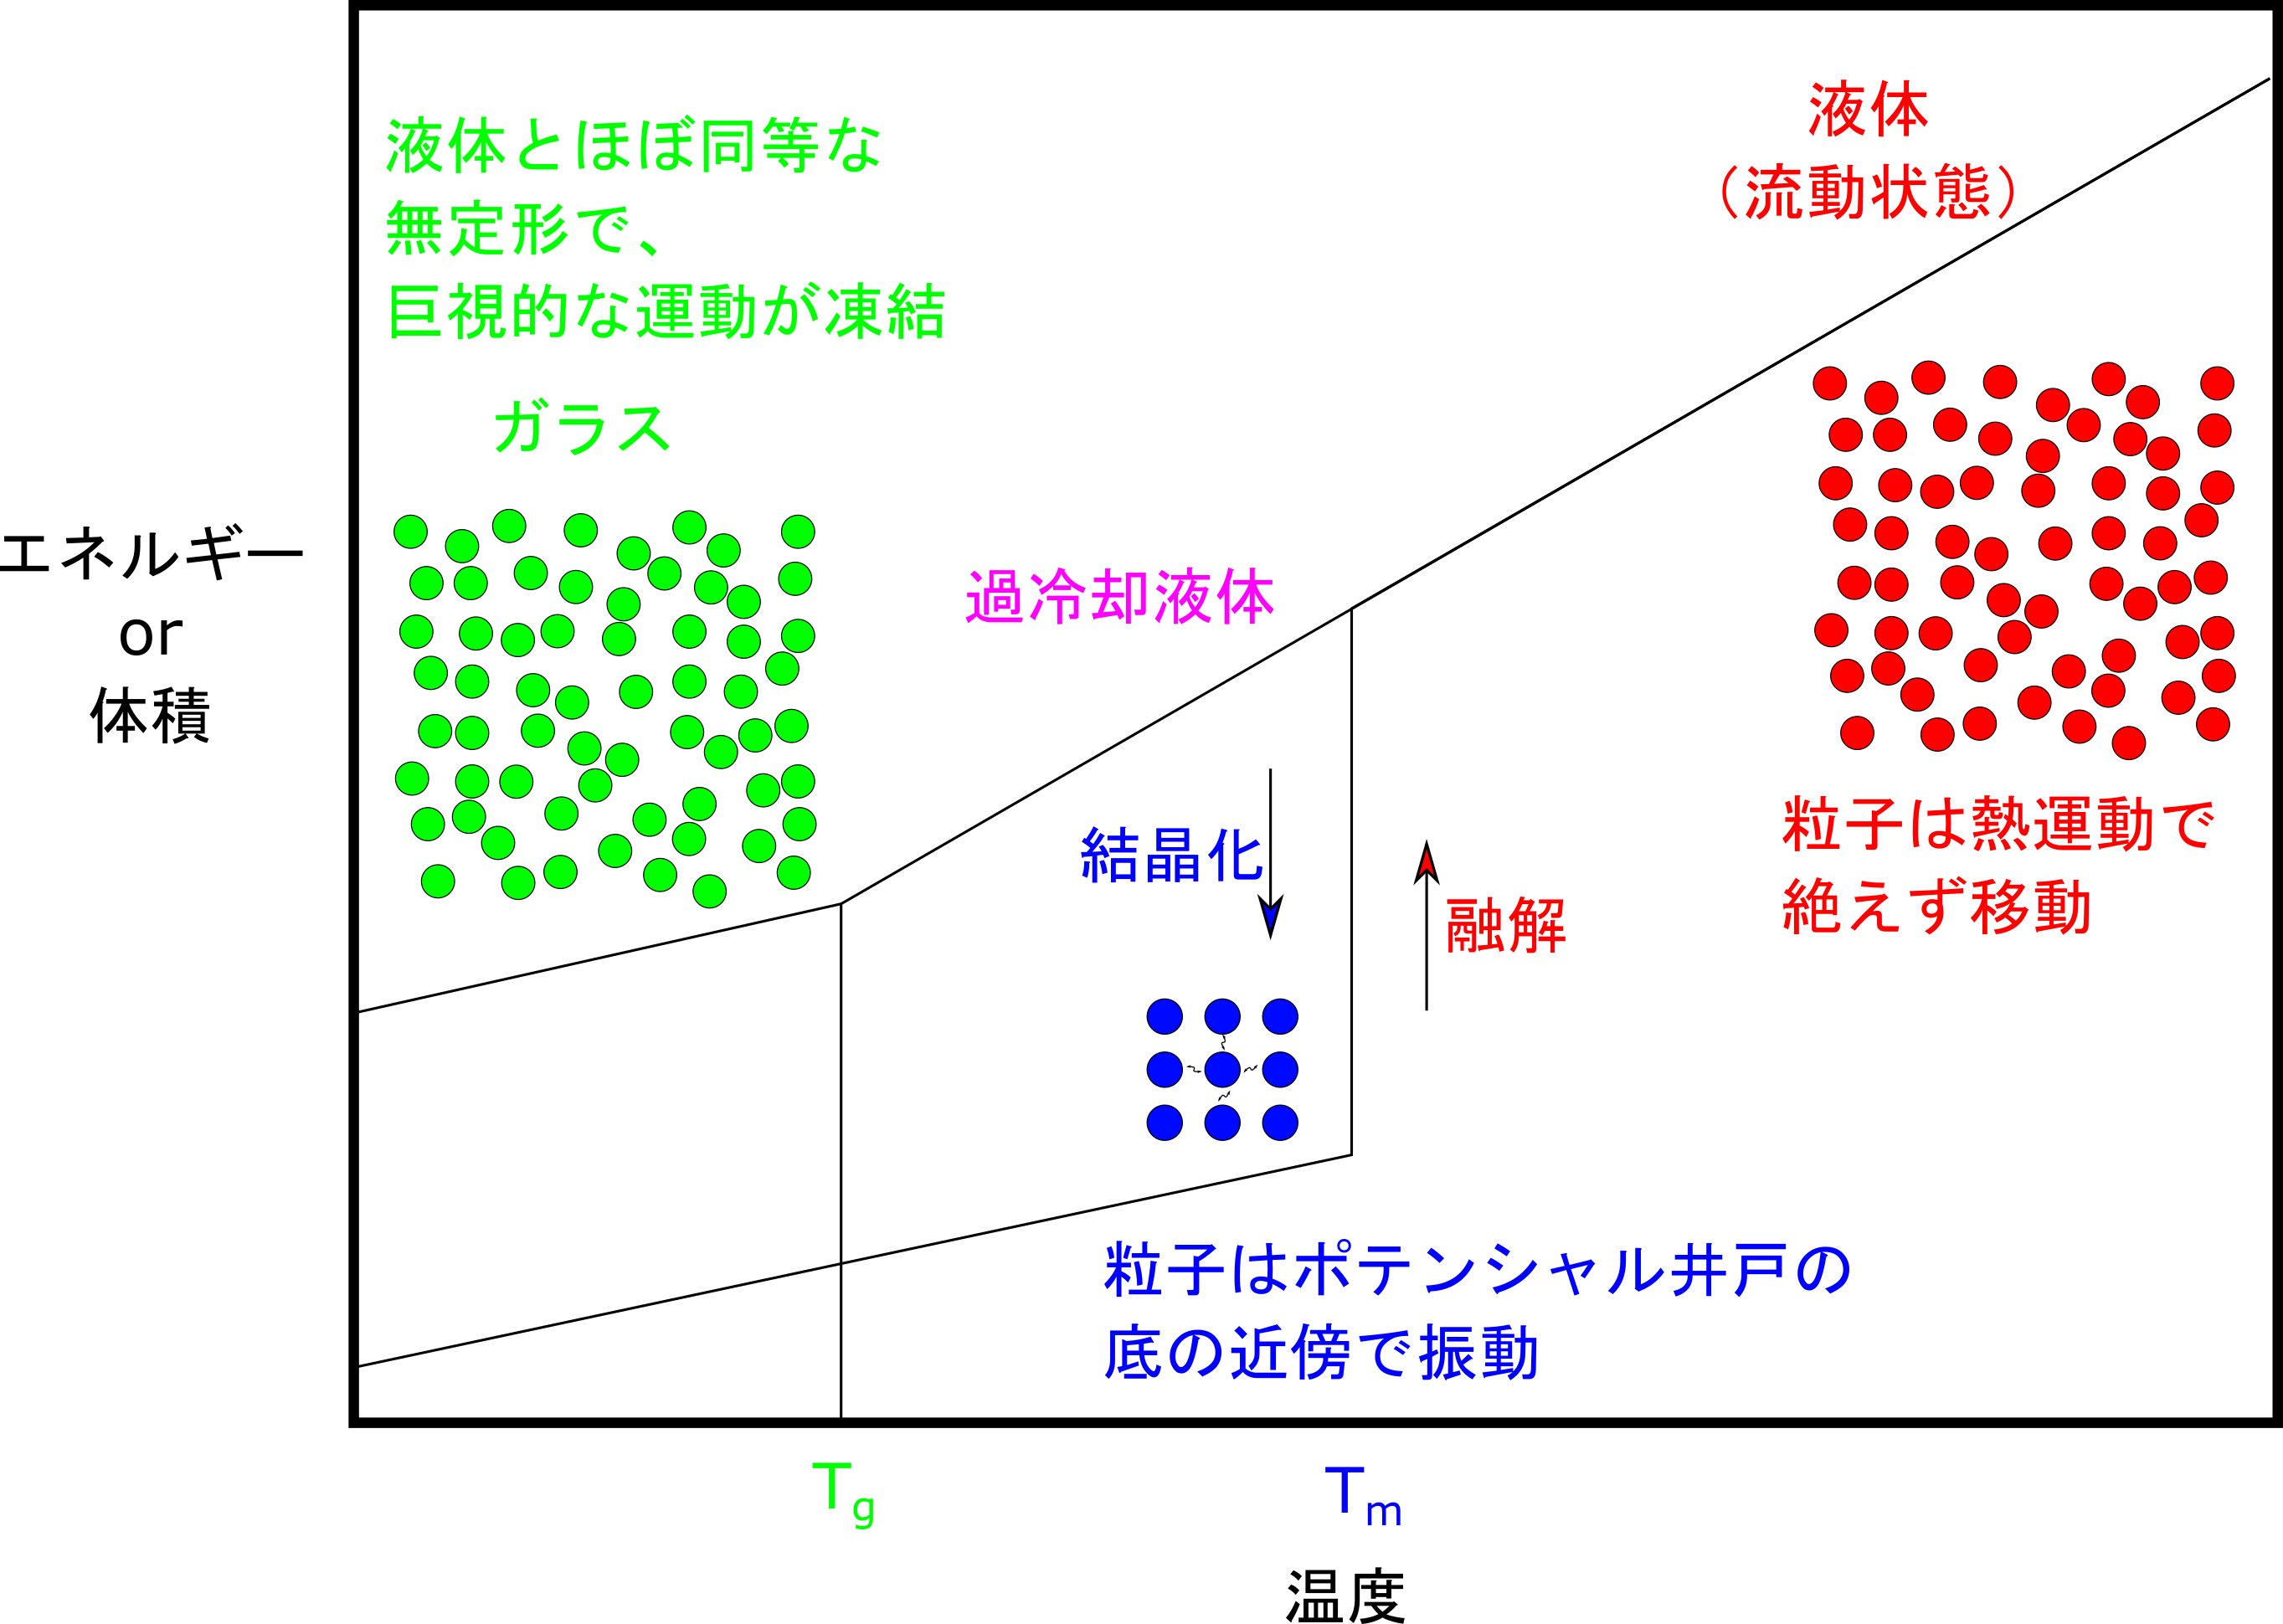
\includegraphics[width=.9\textwidth]{glass_trans.png}
			\end{center}
		\end{minipage}
		\caption{ガラス転移とガラス状態}
		\label{fig:glass}
	\end{center}
\end{figure}

図 \ref{fig:glass} に示したように、液体\index{えきたい@液体}からガラスへと変化する際には、結晶化とは異なり体積に飛びを生じることなくガラスへの転移に伴い傾きの変化が生じます。ただ、比熱には違いが生じますが結晶化のような一定温度での飛びとは異なり滑らかな変化となる場合が多い。 

\subsubsection{ガラス転移について}

ガラス転移について、もう少し考えてみましょう。

直感的には、単純な粒子であれば並びやすいことは容易にイメージできるでしょう。
一方、複雑な形状を有する粒子ではそのぞれの粒子同士の並び方に選択肢が多くて、逆に、全部が同じように並ぶ状態を取りにくいということも、なんとなく想像できると思います。

例えば、ポリマーというビーズが沢山連なりヒモ状となったような巨大分子は、非晶質でガラス化することが知られています。

\subsubsection{ポリマーのガラス転移の例}

ポリマーがガラス転移するという現象を、ビーズが2つ繋がった最も単純な構造のポリマーで確かめてみましょう。

分子動力学シミュレーションで、ビーズが2つのポリマーを液体\index{えきたい@液体}状態の高温から少しずつ冷却していきます。
高温側の傾きのきつい領域が液体\index{えきたい@液体}です。
T = 0.46近傍で、体積の飛びを示すことなくガラス化が生じています。
それより低温の傾きがゆるい領域がガラス状態ということになります。
\begin{figure}[htb]
	\begin{center}
		\begin{minipage}{0.45\textwidth}
			\large
			\begin{itembox}[l]{分子動力学シミュレーション}
				\begin{itemize}
					\item ビーズが2つのポリマー
					\item 高温から少しずつ冷却
					\item 傾きのきつい領域が液体
					\item 体積の飛びを示すことなく\\ガラス化
					\item 傾きがゆるい領域がガラス
				\end{itemize}
			\end{itembox}	
		\end{minipage}
		\begin{minipage}{0.45\textwidth}
			\begin{center}
			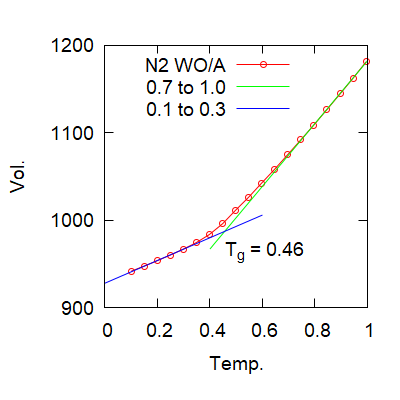
\includegraphics[width=\textwidth]{N2_NoAng_NV_T.png}
			\end{center}
		\end{minipage}
		\caption{ポリマーのガラス転移のシミュレーション}
		\label{fig:polymer_sim}
	\end{center}
\end{figure}

このとき、内部のミクロな状態はどうなっているのでしょうか。

図 \ref{fig:polymer_glass}に、液体状態(T = 1.0)とガラス状態(T = 0.1)の両方のシミュレーションのスナップショットを示しました。
この絵を見ているだけでは、どちらがどちらかの見分けはつかないと思います。
図の下のリンクをクリックしていただければ、それぞれの状態の動画を確認することができます\footnote{
	紙ベースでは、\url{https://drive.google.com/file/d/1V5lLeoqhoUcujVnHqEzFumDlGXC_rPe-/view?usp=sharing}\\
	および、\url{https://drive.google.com/file/d/1HBZ6eQQp0o2vft4bUGxRJUwv4vabs_7d/view?usp=sharing}
}。

ガラス状態における非晶とは、このように液体\index{えきたい@液体}と同等な並び具合を持って、それぞれの粒子\index{りゅうし@粒子}が動けなくなっている状態なのです。
また、それぞれの粒子\index{りゅうし@粒子}は、その雰囲気温度に対応する程度の摂動(安定な状態の近くでの微小な運動)は生じています。
このような状況をイメージすることができれば、ガラス状態のものが長時間の観察において少しずつ流動するということもなんとなく納得できると思います。
\begin{figure}[htb]
	\begin{center}
		\begin{minipage}{0.45\textwidth}
			\large
			\begin{itemize}
				\item 液体状態(T = 1.0)

				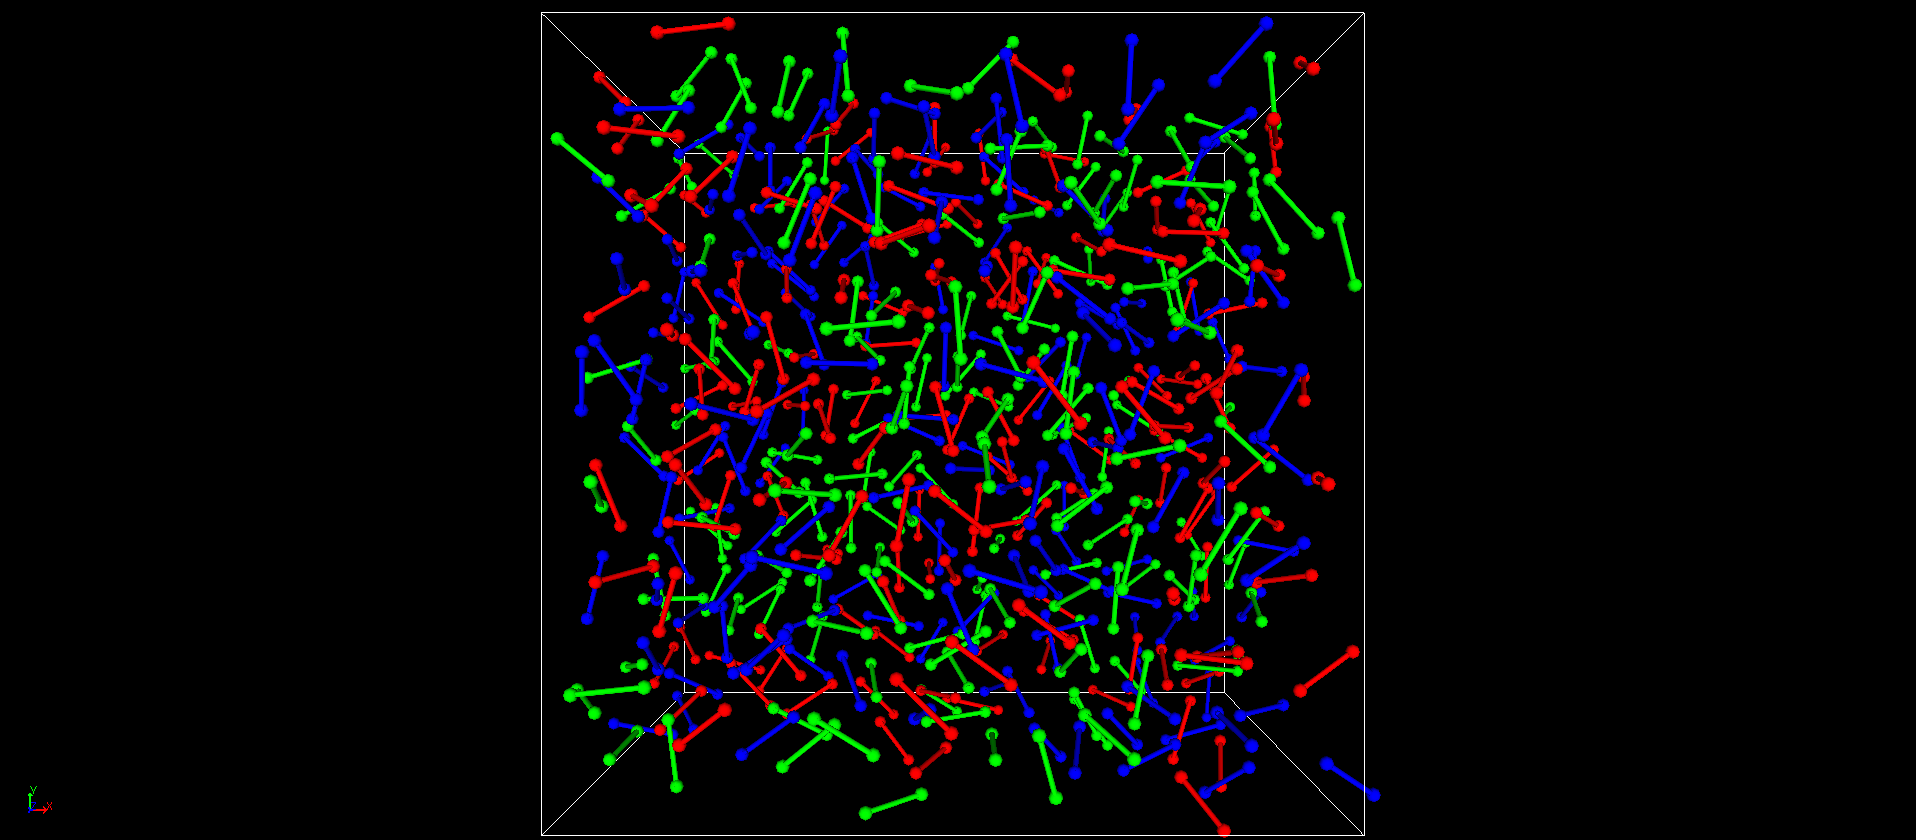
\includegraphics[width=.95\textwidth]{N2_T_1.png}
				\item \href{https://drive.google.com/file/d/1V5lLeoqhoUcujVnHqEzFumDlGXC_rPe-/view?usp=sharing}{液体状態の動画へのリンク}
			\end{itemize}
		\end{minipage}
		\begin{minipage}{0.45\textwidth}
			\large
			\begin{itemize}
				\item ガラス状態(T = 0.1)

				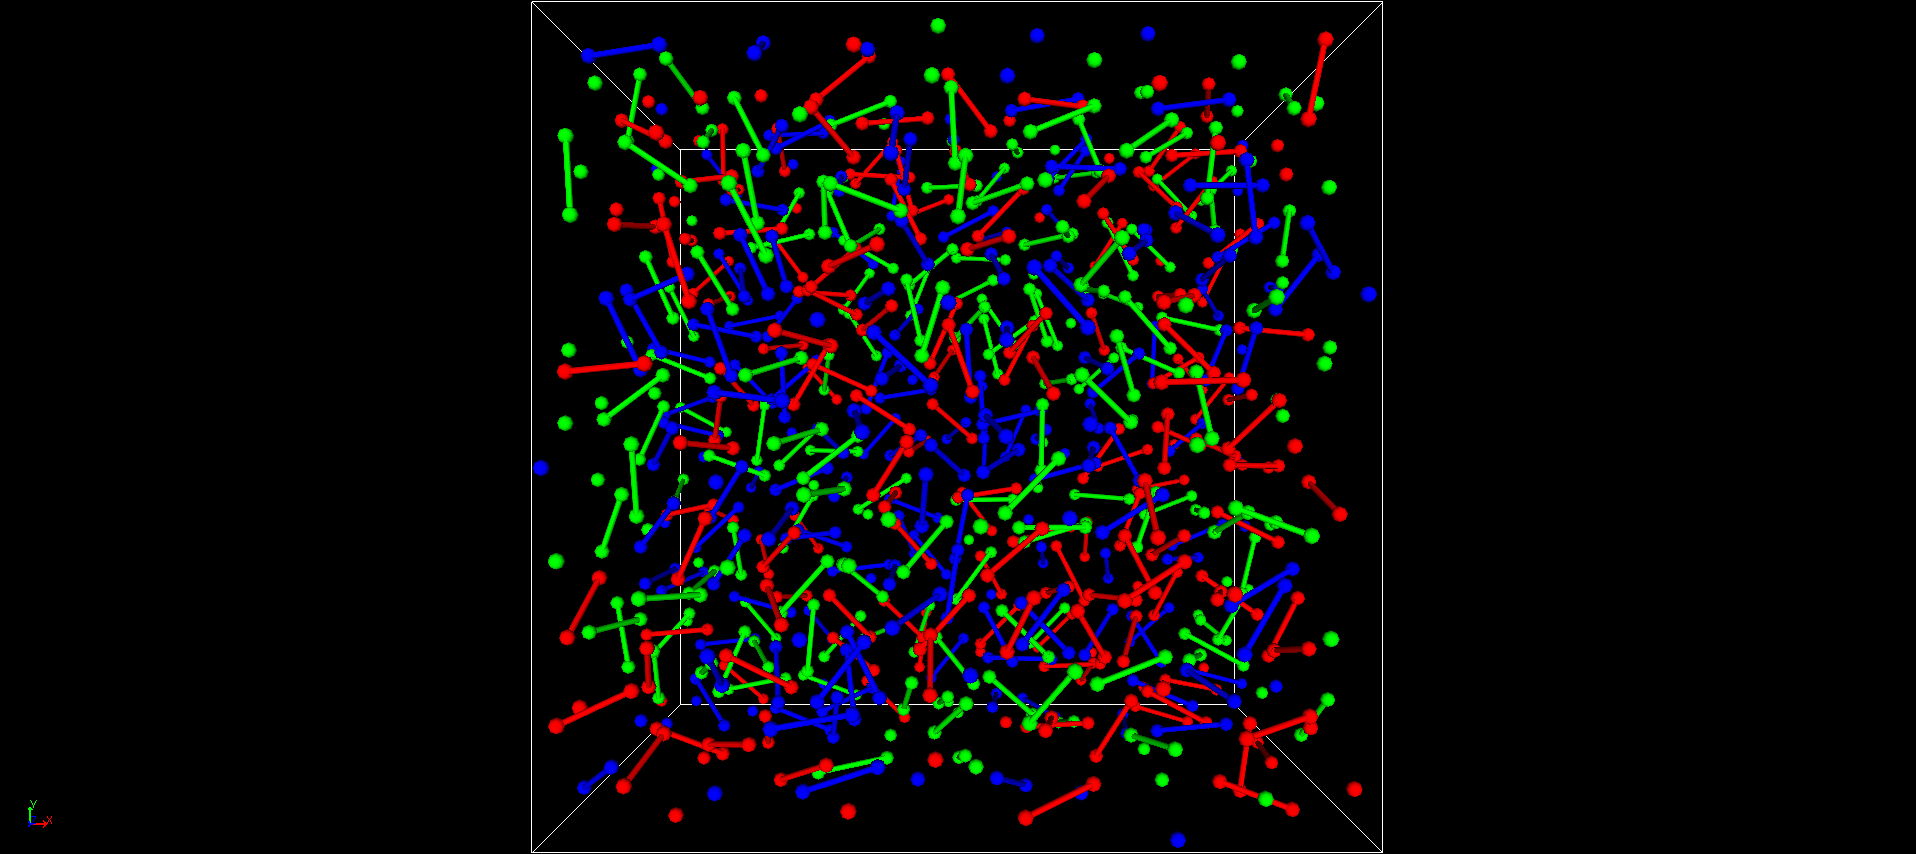
\includegraphics[width=.95\textwidth]{N2_T_0_1.png}
				\item \href{https://drive.google.com/file/d/1HBZ6eQQp0o2vft4bUGxRJUwv4vabs_7d/view?usp=sharing}{ガラス状態の動画へのリンク}
			\end{itemize}
		\end{minipage}
		\caption{シミュレーションでみた液体とガラスの内部状態の比較}
		\label{fig:polymer_glass}
	\end{center}
\end{figure}



\section{応力の由来は?}

ここでは、応力\index{おうりょく@応力}の由来についての考察を進めていきます。

「物質の変形と応力\index{おうりょく@応力}」についての以前の議論をもう一度思い出しましょう。
物質を変形させると、物質はひずんで内部で応力\index{おうりょく@応力}が発生するのでした。

なお、ここでの変形は線形応答となるような微小な変形を考えます。
したがって、その時の系の応答である応力は、重ね合わせの適応できる理想的なものとなります。


\subsection{物質の変形と応力\index{おうりょく@応力}}

そのような応力について、固体\index{こたい@固体}と液体\index{えきたい@液体}の違いを考えます。

ここまでの議論での固体\index{こたい@固体}は、単純な固体を考えていますので内部でも一様に変形すると考えて、生じる応力が一様となります。

一方、液体\index{えきたい@液体}の場合は、変形を止めれば応力も消失すると考えます。
このとき、液体内部では、粒子同士の相互作用\index{そうご@相互作用}が増加しているのですが、粒子\index{りゅうし@粒子}が移動すれば増加分が消失してしまいます。
\large
\begin{itembox}[l]{固体と液体の違い}
	\begin{itemize}
		\item 固体では
		\begin{itemize}
			\item 単純な固体は一様に変形すると考えて、
			\item 生じる応力が一様で持続的
		\end{itemize}
		\item 液体の場合
		\begin{itemize}
			\item 変形を止めれば、応力も消失すると考える。
			\item このとき、液体内部では、
			\begin{itemize}
				\item 粒子同士の相互作用が増加
				\item 粒子が移動すれば、増加分が消失
			\end{itemize}
		\end{itemize}
	\end{itemize}
\end{itembox}
\normalsize

\subsection{結晶の応力の起源}

では、固体\index{こたい@固体}のモデルとして結晶の応力\index{おうりょく@応力}の起源について考えましょう。

結晶にマクロな変形を与えると、固体内部でもミクロに変形が生じます。
このとき、マクロと相似にミクロな変形が生じるものと単純化して考えます。
そして、そのミクロな変形の結果として、粒子間でも安定位置からの変位が生じるわけです。
なお、このミクロな変位は同一とは限りませんから、粒子間は接近するものもありますし、離れるものも生じます。

このミクロな安定な位置からの変位を、局所的に二体間のポテンシャル\index{ぽてんしゃる@ポテンシャル}で考えると以下のような力が生じます。
\begin{itemize}
	\item 接近した場合は、 $\Leftrightarrow$ 斥力
	\item 離反した場合は、 $\Leftrightarrow$ 引力
\end{itemize}

局所的な上記のミクロな力の積分\index{せきぶん@積分}値として、マクロな応力が発生すると考えることができます。

\begin{figure}[htb]
	\begin{center}
		\begin{minipage}{0.45\textwidth}
			\large
			\begin{itembox}[l]{マクロな変形の付与により}
				\begin{itemize}
					\item 固体内部でもミクロに変形
					\item マクロと相似に変形と単純化
					\item 粒子間で安定位置から変位
				\end{itemize}
			\end{itembox}
			\begin{center}
				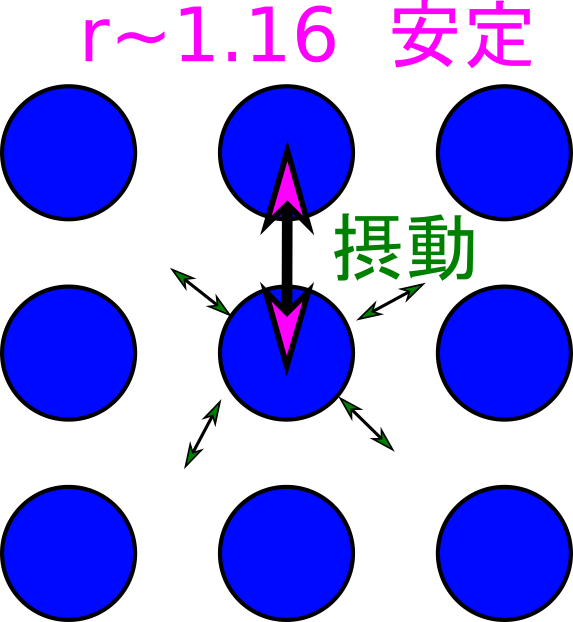
\includegraphics[width=.58\textwidth]{LJ_ryusi.png}
			\end{center}
		\end{minipage}
		\begin{minipage}{0.45\textwidth}
			\large
			\begin{itembox}[l]{ミクロに安定な位置から変位}
				\begin{itemize}
					\item 局所的には二体間で考えると、
					\begin{itemize}
						\item 接近した場合は、 $\Leftrightarrow$ 斥力
						\item 離反した場合は、 $\Leftrightarrow$ 引力
					\end{itemize}
					\item その積分値として、マクロな応力が発生
				\end{itemize}
			\end{itembox}
			\begin{center}
				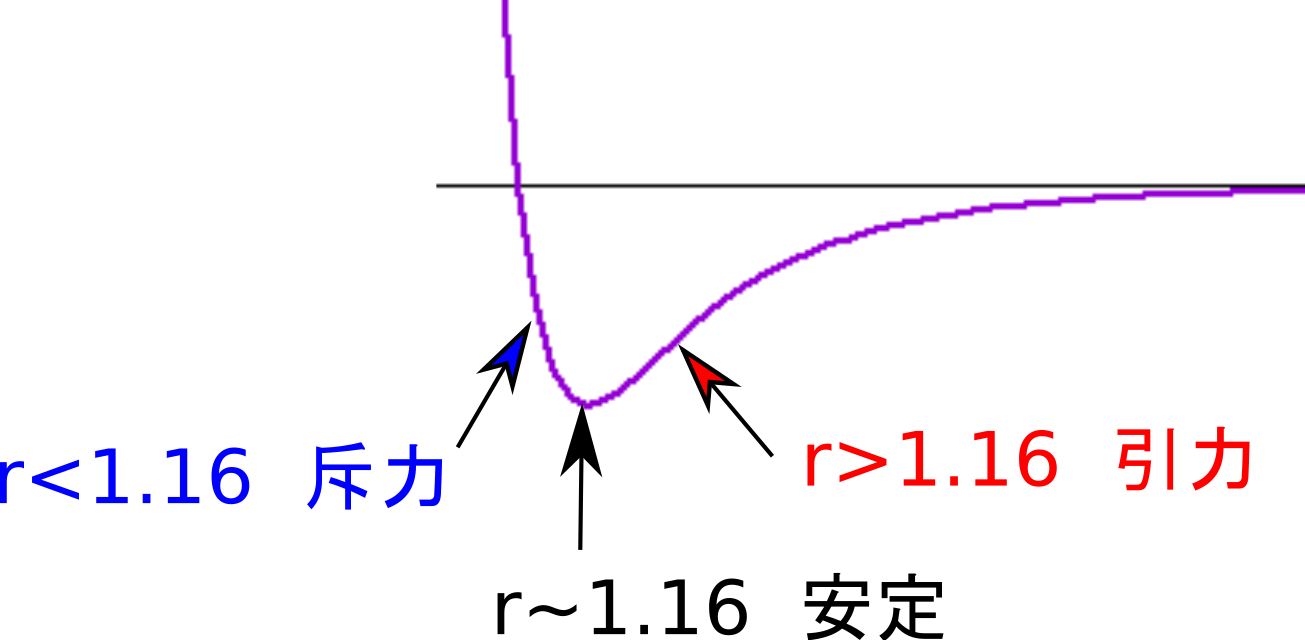
\includegraphics[width=\textwidth]{LJ_pos.png}
			\end{center}
		\end{minipage}
		\caption{結晶の応力の起源について}
		\label{fig:stress_crystal}
	\end{center}
\end{figure}

\subsection{液体\index{えきたい@液体}の応力\index{おうりょく@応力}とは?}

つぎに、液体\index{えきたい@液体}の応力\index{おうりょく@応力}についてです。

前述のように、液体\index{えきたい@液体}の場合は変形を止めれば応力も消失しますから、ここでの議論では変形を与えた瞬間のことを考えます。
瞬間的に考えれば、液体においても固体\index{こたい@固体}と同様にマクロな変形に対応してミクロな変形が生じることになります。
ただ、このとき、結晶の状況と異なるのは、粒子\index{りゅうし@粒子}が規則的に並んでいるわけではないということです。
\begin{figure}[htb]
	\begin{center}
		\begin{minipage}{0.45\textwidth}
			\large
			\begin{itembox}[l]{マクロな変形}
				\begin{itemize}
					\item マクロにせん断変形を付与
					\begin{itemize}
						\item ミクロにも粒子近傍が変形
					\end{itemize}
					\item 一粒子に着目すると、
					\begin{itemize}
						\item ポテンシャル場が変化
						\item 局所的に「歪んだかご」
						% \item 「歪んだかご」の中で、\textcolor{red}{居心地が悪くなる。}
						% \item その結果として\textcolor{red}{局所的な応力が発現}
					\end{itemize}
				\end{itemize}
			\end{itembox}
			\begin{center}
				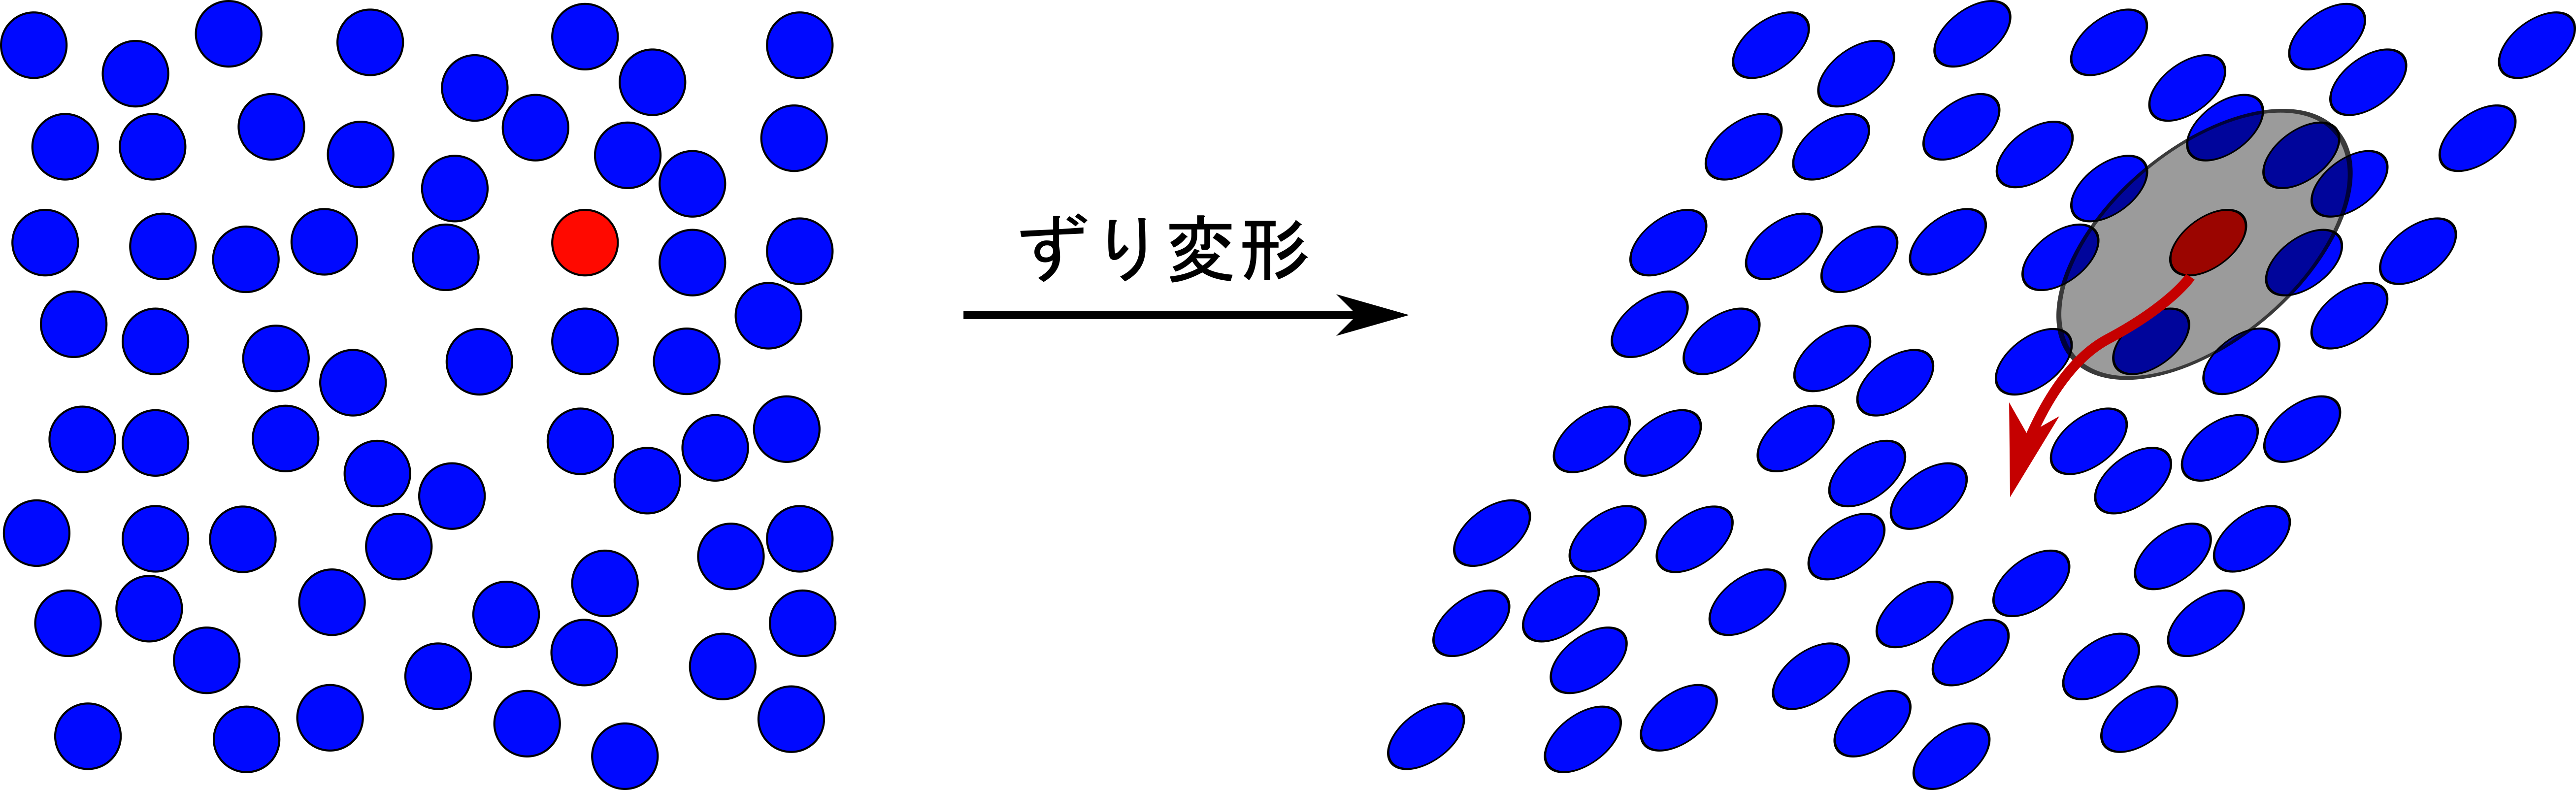
\includegraphics[width=.9\textwidth]{liquid_flow.png}
			\end{center}
		\end{minipage}
		\begin{minipage}{0.45\textwidth}
			\large
			\begin{itembox}[l]{ミクロな応力から流動へ}
				\begin{itemize}
					\item 「歪んだかご」の結果、
					\begin{itemize}
						\item \textcolor{red}{粒子の居心地が悪化}
						\item \textcolor{red}{局所的な応力が発現}
						\item 積分値としてマクロな応力
					\end{itemize}
					\item 「歪んだかご」からの脱出
					\begin{itemize}
						\item ミクロな応力が消失
					\end{itemize}
					\item マクロにも流動\index{りゅうどう@流動}
					\begin{itemize}
						\item マクロな応力も消失
					\end{itemize}
				\end{itemize}
			\end{itembox}
		\end{minipage}
		\caption{液体の応力の起源について}
		\label{fig:stress_liquid}
	\end{center}
\end{figure}

したがって、一粒子に着目した場合、その粒子\index{りゅうし@粒子}と他の粒子\index{りゅうし@粒子}との距離は均一ではなく、その状態からさらにひずみ\index{ひずみ@ひずみ}が与えられます。
このとき、この粒子\index{りゅうし@粒子}は局所的に「歪んだかご\index{ひずんだ@歪んだかご}」に閉じ込められたということになり、居心地が悪い状態\footnote{
	この表現は、イメージとしてのモデル的なものであり、熱力学をご存知な方には自由エネルギーが上昇したと捉えていただければと思います。
}になります。
その結果として、局所的にミクロに見た応力が発生するわけです。
そして、固体と同様に、その積分値として瞬間的なマクロな応力へとつながります。

液体\index{えきたい@液体}の場合は、それぞれの粒子\index{りゅうし@粒子}は熱運動していますから、多少の時間経過に伴いこの着目した粒子は「歪んだかご\index{ひずんだ@歪んだかご}」から脱出できます。
そして、ミクロな応力\index{みくろ@ミクロな応力}が消失しますし、かごからの脱出によって粒子\index{りゅうし@粒子}の異方的な移動が生じますから、マクロにも流動することになり、マクロな応力も消失します。

\section*{この章のまとめ}
この章では、物質の三態(固体、液体、気体)という最も基本的な「ものの有り様」について、物理化学的に⾒直しました。
\begin{boxnote}
	\large
    \begin{itemize}
		\item 物質の三態について
		\begin{itemize}
			\item 固体のモデルとして、粒子が規則的に並んだ結晶を用いて議論し、
			\item 液体のモデルについては、シミュレーションも交えてイメージを深めた。
		\end{itemize} 
		\item 流れるということは?
		\begin{itemize}
			\item マクロな変形と粒子の移動の関係についてのイメージを示し、
			\item 固体と液体の境目が曖昧であって、
			\item ガラス状態という中間的な状態があることを示した。
		\end{itemize} 
		\item 応力の由来は?
		\begin{itemize}
			\item 結晶の応力の起源について、粒子描像をベースに相互に安定な状態にあることを示し、
			\item 液体の応力は、「歪んだかご」からの脱出の際に生じるが、流動\index{りゅうどう@流動}により消失することを示した。
		\end{itemize}
	\end{itemize}
\end{boxnote}

\newpage

\begin{longartdeco}
	\begin{center}
	\emph{コラム:抽象と捨象}	
	\end{center}

	普段の会話において、「あなたの話は抽象的すぎて実感しにくいから、もっと具体的に話して」と言われてしまうことがたまにあります。
また、「抽象画」として分類される「一見しただけではなんだかよくわからない絵」と感じられる作品に対して、ネガティブなイメージを持つ方もいるようです。
この2つの例が示すものは、抽象するという行為が、作者(話者)の独りよがりであり、「私に容易に理解できないから、あまりいいやり方ではないでしょ」というような否定的な感覚かもしれません。
しかし、抽象的であることは、「普通の人はやらない、良くないやり方」なのでしょうか?

例えば、著名なピカソの絵画(キュービズムというように分類されるようです)を考えてみましょう。
彼の絵画は、幼少期には卓越した表現力(9歳のときのデッサンがすごい)を持った写術的なものであったのに、青の時代、バラ色の時代、アフリカ彫刻の時代と呼ばれる3つの変遷を経て、泣く女やゲルニカのような不思議な世界へと発展していきます。
この「キュービスム」とは、人や自然の立体的な風景を全て複数の視点から見た幾何学的な形で捉え、平面にそのまま表す様式です。
これは、私たちが普段、ものを一つの視点からしか見ることができていないのとは大きく異なっています。
多様な視点を同時に描くというアプローチ(キューブ:立方体を同時に全部の面を描く)によって、見る側の視点を超えた、「物や人の本質に迫ろう」とし、より「純粋な絵画」を目指したと考えられています。

また、我々が、抽象的な話をするときというのは、「理想」とか「あるべき姿」や「真理」のような手にとって見ることができない(形而上の)事柄を議論するときがほとんどです。
「理想」や「真理」を具体的にと言っても、無理な話ですよね。

そもそも、「抽象とは大事なことを抽き出す」ことです。
星の王子さまも言っているように「いちばんたいせつなことは、目に見えない」し、人はつい、「きみはごちゃ混ぜにしてる……大事なこともそうでないことも、いっしょくたにしてる!」という状況になってしまうから、大事なことを探し出さなくてはいけないのです。
また、類似の行為を表す言葉として、「捨象」というものもあります。
こちらは、本質を探るために「いらない部分を捨てる」行為ですから、ある程度「たいせつなもの」が見えてきたときに有用な行為となるでしょう。

\end{longartdeco}


\end{document}